\subsection{Replication}
\subsubsection{Partial Replication: Testing prior findings}

The foundation of any replication study is fidelity—ensuring that the methodological and analytical choices align as closely as possible with the original study. In this section, our primary goal is to faithfully replicate the methodological choices of \citep{Ge2021}, ensuring that our analyses align with the original study’s design, statistical procedures, and reporting conventions. Fidelity in a replication serves as a critical foundation for scientific transparency, allowing us to assess whether the original findings hold under comparable conditions. Given the shift to web-based data collection, maintaining methodological consistency is essential to isolate potential differences due to changes in modality from those due to variations in statistical approach or participant characteristics.

To achieve this, we adhere as much as possible to the original pre-processing steps, statistical models, and analytical decisions outlined in \citep{Ge2021}. This includes using the same data transformations and inferential techniques to ensure that our replication remains as close as possible to the original study. Any unavoidable deviations, whether due to differences in implementation, data collection platform, or sample composition, are explicitly documented to clarify the degree to which methodological fidelity has been maintained.

Following \cite{Ge2021}, we analyzed fixation proportions to target objects, object-stressed competitors, verb-stressed competitors, and distractors across time, comparing conditions in which the object or verb was stressed. To maintain fidelity, we used a comparable time-binning approach, aligned with the beginning and end of each word in the sentence (e.g., ``The rabbit is", ``only", ``verb1", ``the1", ``object1", ``gap", ``not", ``verb2", ``the2", ``object2", ``offset"). This follows \cite{Ge2021}’s critical word boundaries and allows for direct comparisons between studies with nine critical time bins. We calculated mean fixation proportions and standard errors for each interest area across time bins and conditions. Like \cite{Ge2021}, we plotted these fixation patterns using a time-series approach, with separate visualizations for each competitor type and experimental group. English fixation proportions across areas of interest (AOI) for both our study and and estimated result of \cite{Ge2021} can be found in Figure \ref{fig:english_fix}; Dutch fixation proportions can be found in Figure \ref{fig:dutch_fix}.

\begin{figure}[H]  % 'p' puts it on its own page
    \centering
    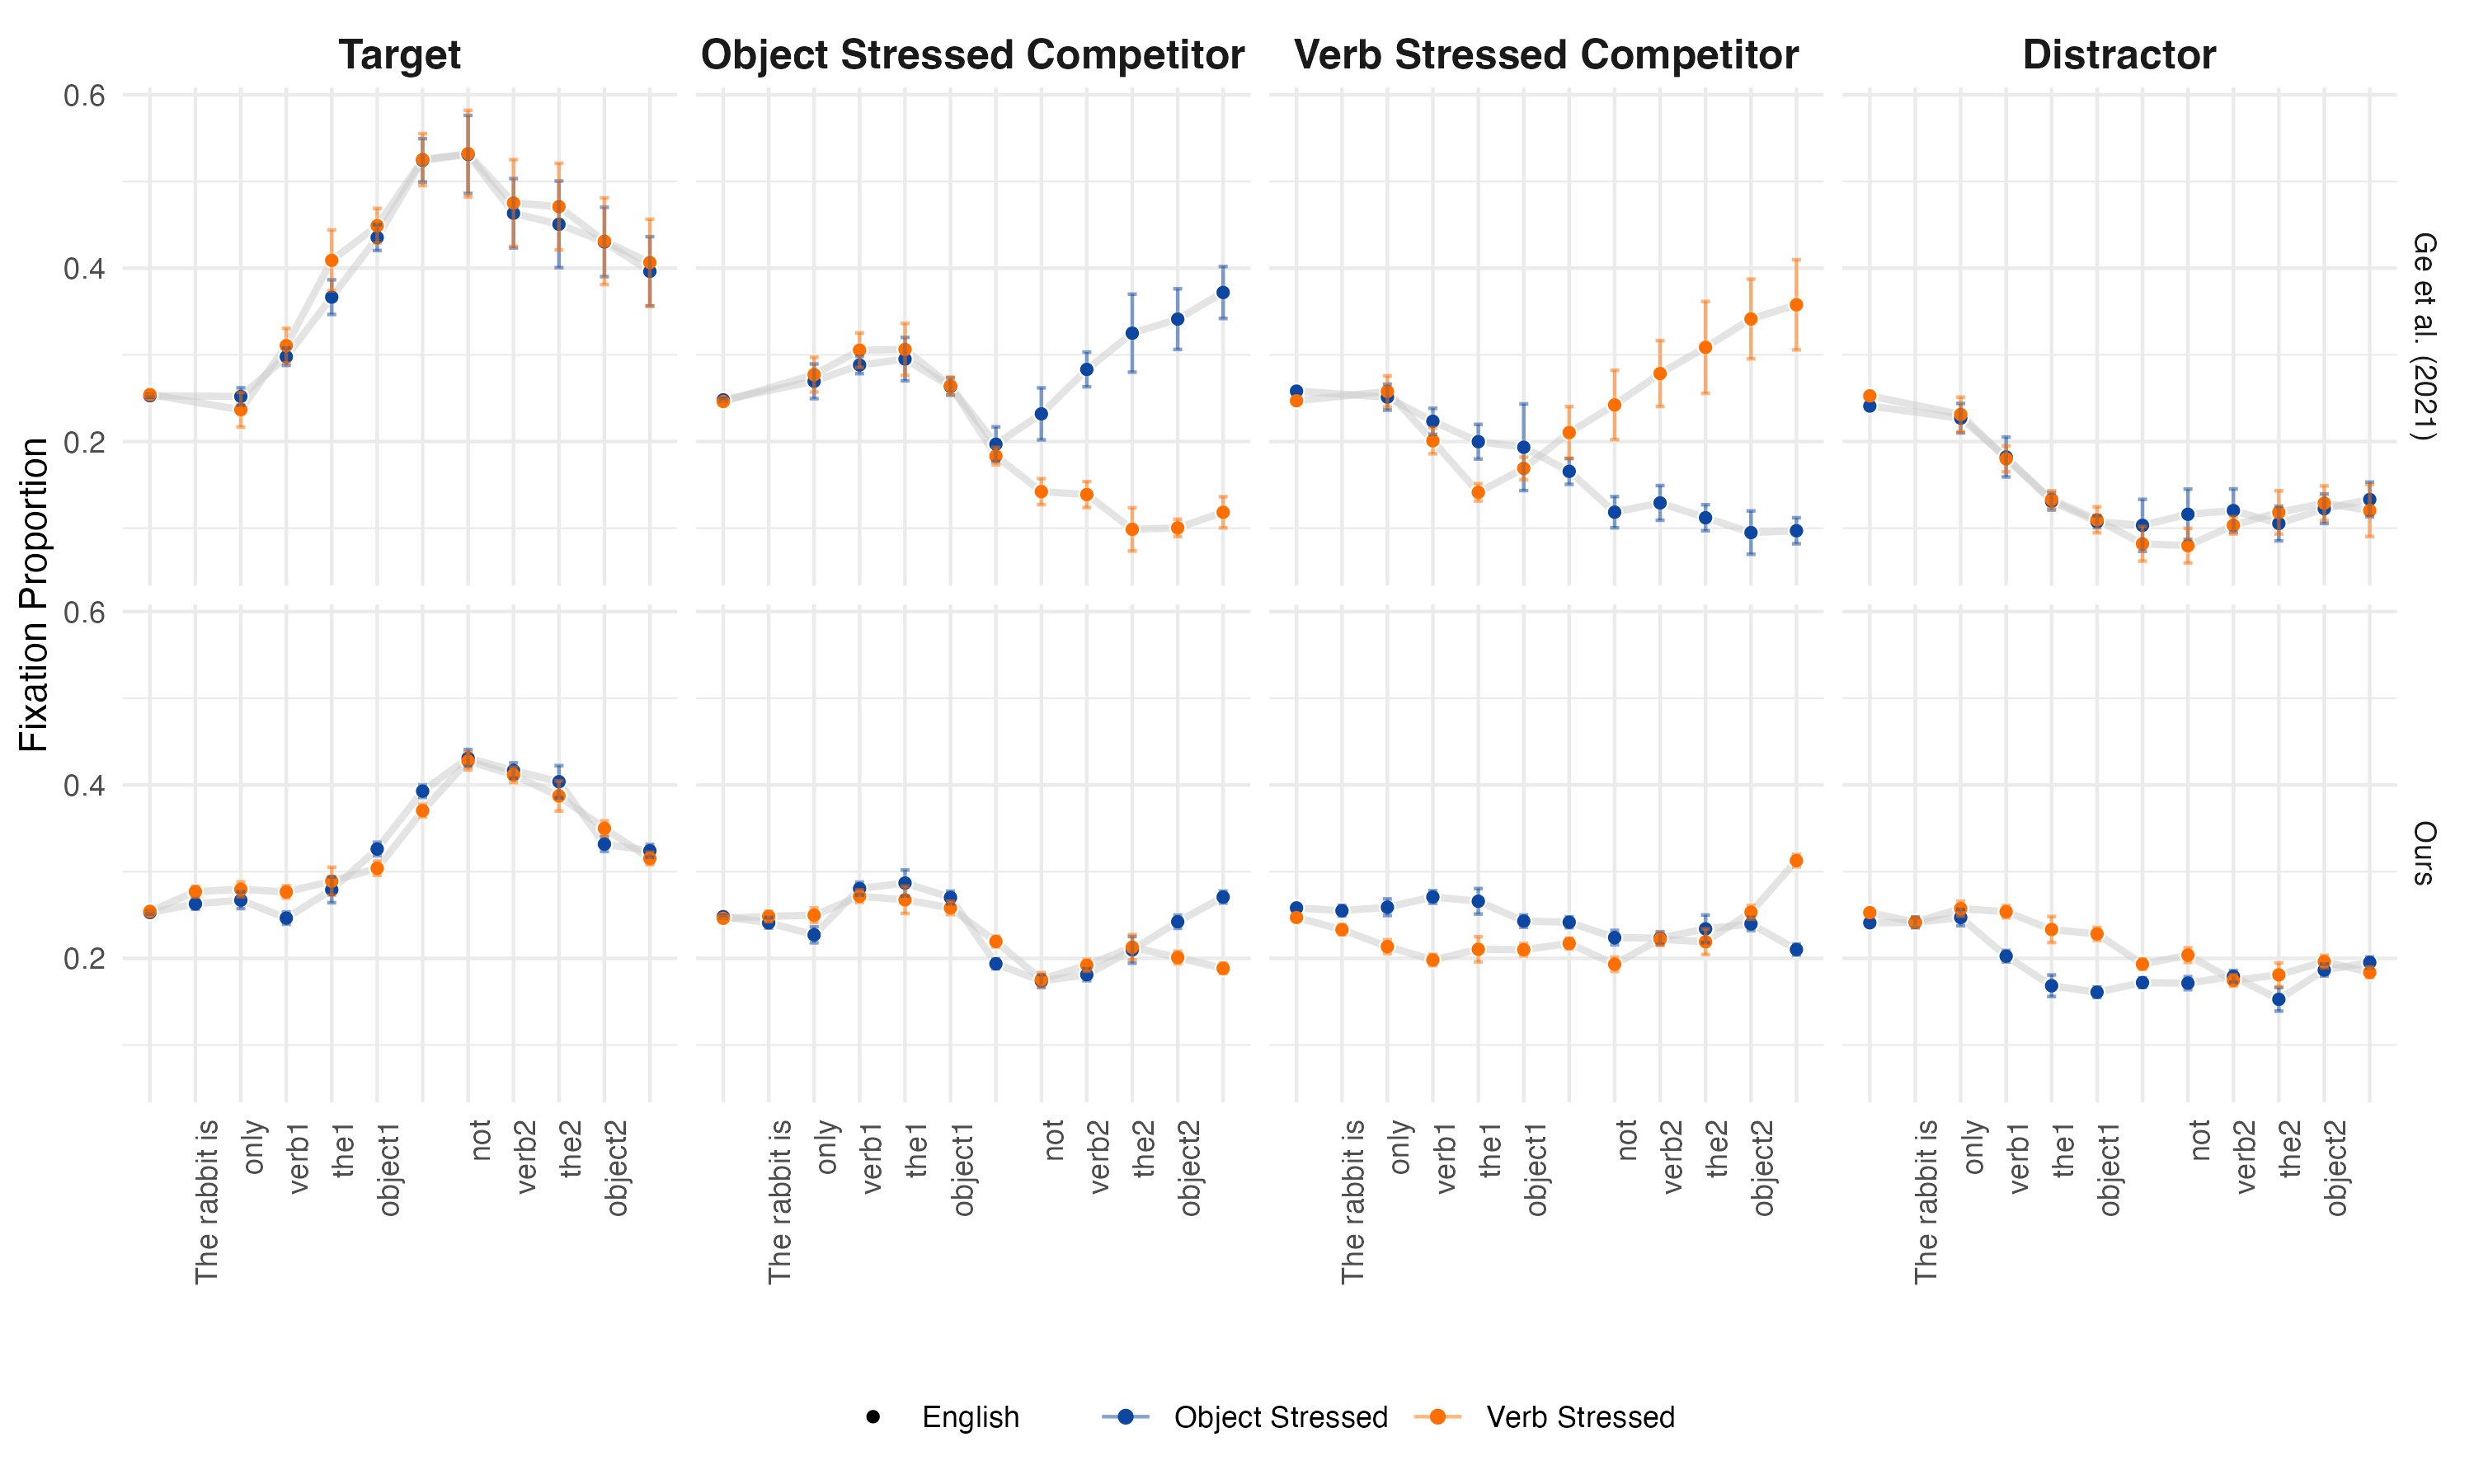
\includegraphics[width=\textwidth,height=\textheight,keepaspectratio]{viz/english_fix.png}
    \caption{L1 English speakers' fixation proportions across time bins from Ge et al. (2021) (top row) and our study (bottom row) by target, competitors, and distractor.}
    \label{fig:english_fix}
\end{figure}

\begin{figure}  % 'p' puts it on its own page
    \centering
    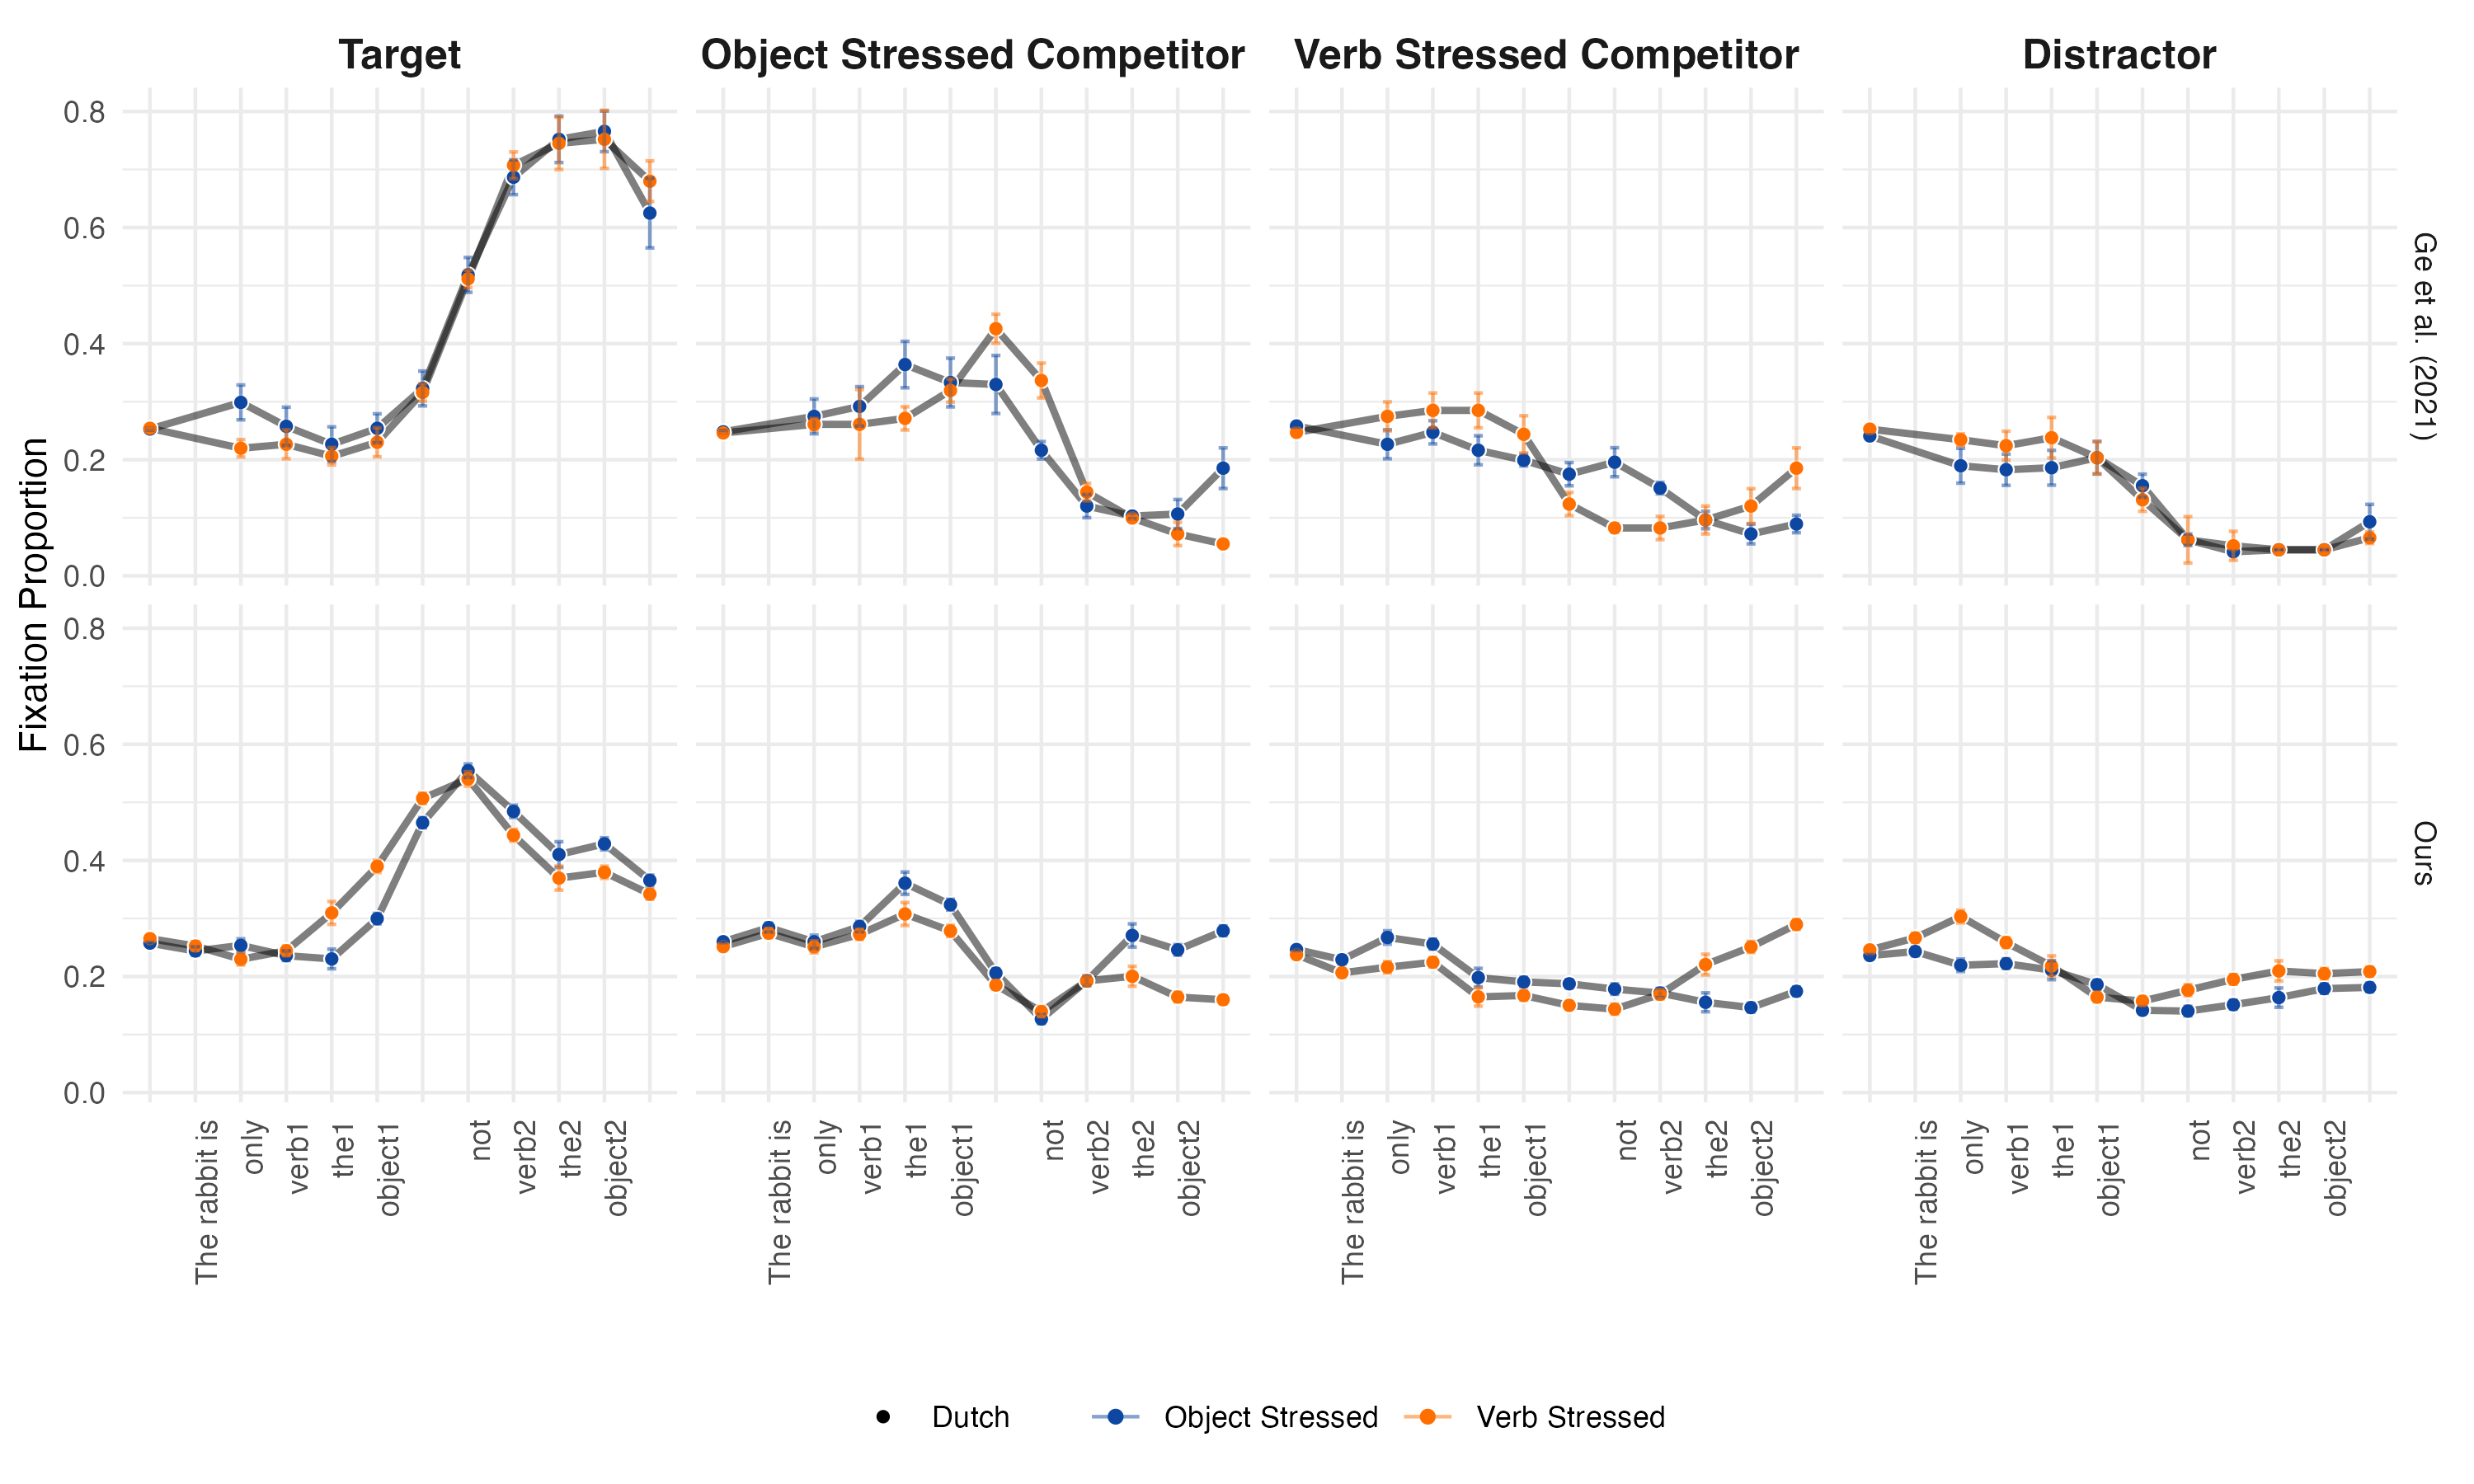
\includegraphics[width=\textwidth,height=\textheight,keepaspectratio]{viz/dutch_fix.png}
    \caption{L1 Dutch-L2 English speakers' fixation proportions across time bins from Ge et al. (2021) (top row) and our study (bottom row) by target, competitors, and distractor.}
    \label{fig:dutch_fix}
\end{figure}

Following \cite{Ge2021}, we applied mixed-effects regression models to predict fixation proportions as a function of focus condition, time, and AOI for each time bin separately. We fit a series of linear mixed-effects models (LMMs) with random intercepts for participants and slopes for condition and AOI. The best-fitting models were selected based on lowest AIC. Following \cite{Ge2021}, we used the baseline of object stressed competitor for condition and a baseline of object stressed competitor for AOI. This means that negative effects for either variable can be interpreted as object facing and positive effects are verb facing. Said another way, a positive effect for AOI means more looks toward verb competitor. Likewise, a positive effect for condition indicates more looks during verb focused sentences.

Unlike \cite{Ge2021}, our model selection pipeline incorporated an automated model comparison approach, iteratively testing models with simpler effects structures. This change was necessary because many models did not converge. The full model included both AOI and condition, along with their interaction, as well as random intercepts for participants and slopes for items. If this failed to converge or created a singularity, then the model was reduced to remove individual slopes but still included the AOI × condition interaction. If that model failed to converge, the AOI x condition interaction was removed, leaving only the main effects. The model was then further simplified by removing participant-specific effects entirely, keeping the overall effects of AOI and condition and participant random slopes. If none of these models converged or if the simplest model was the best, then the last step was a basic linear model without any participant-level adjustments, treating all data points as independent. This yielded 18 statistical tests (9 critical time bins x 2 L1 groups). We present results in order from the beginning of the sentence to the end. 

Starting with the L1 English models, three significant effects were found: A positive effect was found for AOI ($\beta$ = 0.062, \textit{SE} = 0.029, \textit{t} = 2.17, \textit{p} = 0.032) indicating more looks to verb competitors than object competitors during the ``not" time bin. A positive interaction between AOI and condition was found ($\beta$ = 0.175, \textit{SE} = 0.056, \textit{t} = 3.14, \textit{p} = 0.0019) for the ``offset" time bin, indicating that participants began to look more at the verb competitor during the verb focused sentences. Additionally, in the same ``offset" time bin, a negative effect was found for condition ($\beta$ = -0.091, \textit{SE} = 0.039, \textit{t} = -2.30, \textit{p} = 0.022) indicating more looks to competitors during object focused sentences overall during the offset time bin. Our L1 English participants' results can be seen in comparison to \cite{Ge2021} in Figure \ref{fig:model_plot_english}.

\begin{figure}[H]  % 'p' puts it on its own page
    \centering
    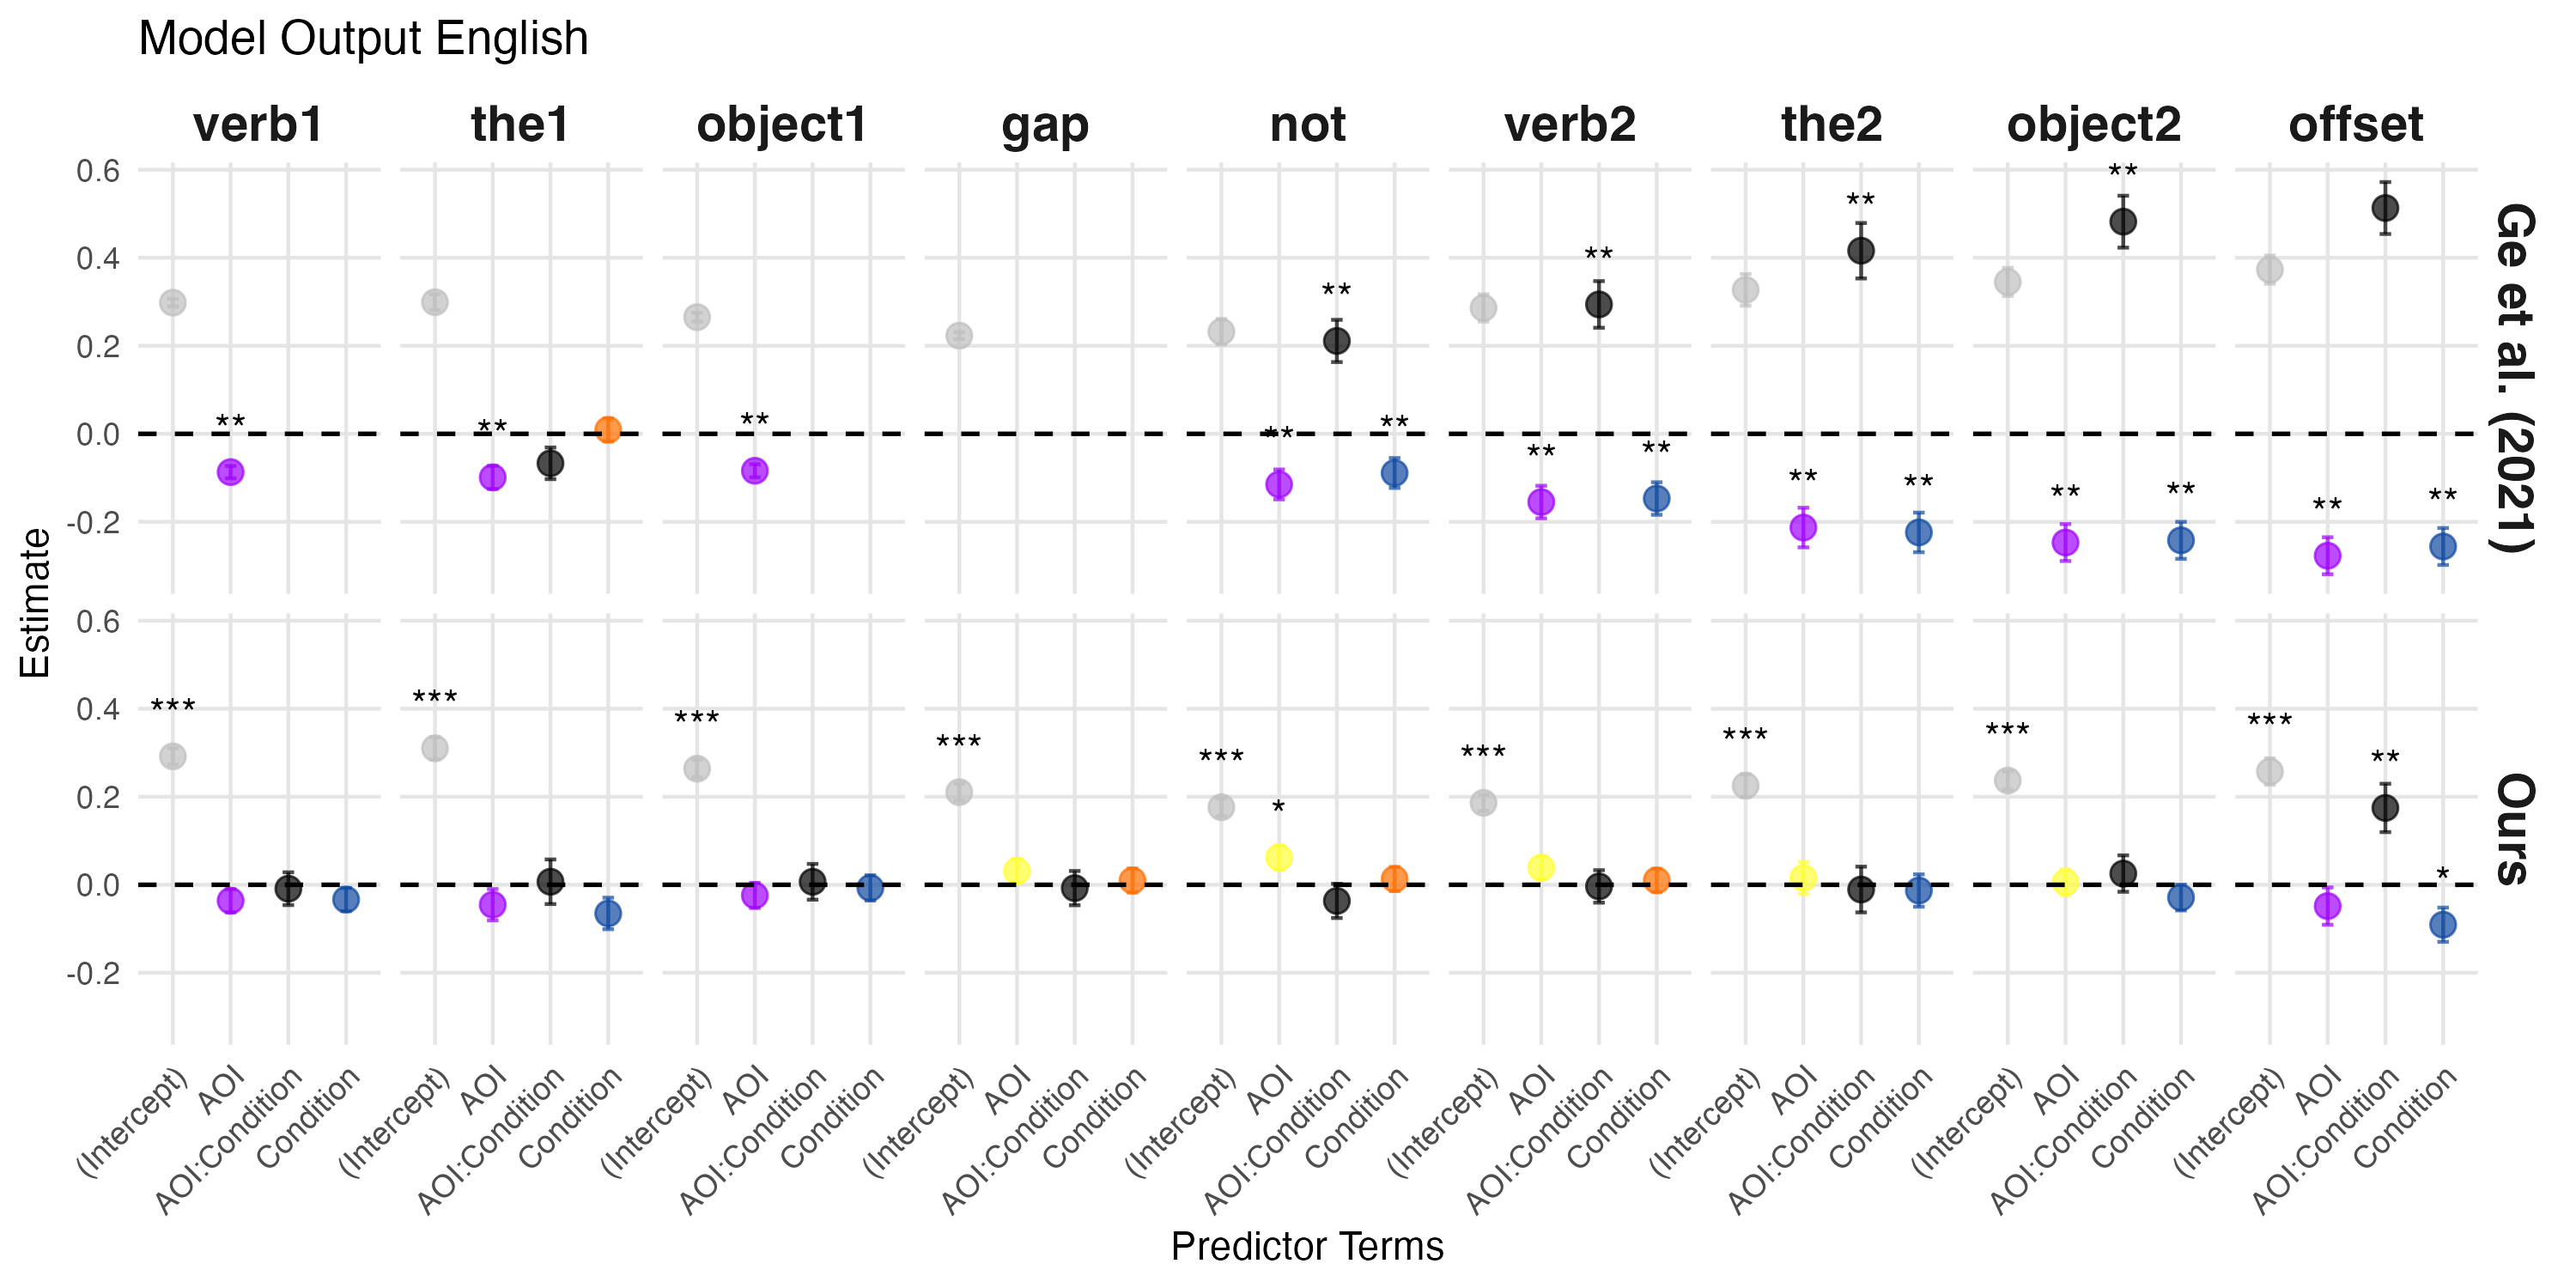
\includegraphics[width=\textwidth,height=\textheight,keepaspectratio]{viz/model_plot_english.png}
    \caption{Model outputs for L1 English participants across nine modeled time bins. Order of time bins appears in order across the top. Estimates of \cite{Ge2021} data appears on top while our data appears below. Significance levels 0.05, 0.01, and 0.001 are indicated by *, **, and ***, respectively above the estimate.}
    \label{fig:model_plot_english}
\end{figure}

For the L1 Dutch-L2 English models, nine significant effects were found: A negative effect of AOI ($\beta$ = -0.099, \textit{SE} = 0.041, \textit{t} = -2.43, \textit{p} = 0.017) was found for ``the" time bin, indicating more looks to object competitor AOIs. Similarly, a negative effect for AOI was found for ``object1" ($\beta$ = -0.117, \textit{SE} = 0.033, \textit{t} = -3.59, \textit{p} $<$ 0.001), ``the2" ($\beta$ = -0.129, \textit{SE} = 0.042, \textit{t} = -3.08, \textit{p} = 0.0025), and ``object2" ($\beta$ = -0.091, \textit{SE} = 0.032, \textit{t} = -2.83, \textit{p} = 0.0055) time bins, all of which indicate more looks to the object competitors AOIs. Further, a negative effect of condition was found for both ``object2" ($\beta$ = 0.180, \textit{SE} = 0.045, \textit{t} = 3.98, \textit{p} $<$ 0.001) and ``offset" ($\beta$ = -0.130, \textit{SE} = 0.050, \textit{t} = -2.58, \textit{p} = 0.011), indicating more looks to competitors during verb focused sentences. Lastly, a positive interaction between AOI and condition was found during the ``object2" ($\beta$ = 0.180, \textit{SE} = 0.045, \textit{t} = 3.98, \textit{p} $<$ 0.001) and ``offset" ($\beta$ = 0.226, \textit{SE} = 0.071, \textit{t} = 3.17, \textit{p} = 0.0019) time bins, indicating more looks to object competitors during object focused sentences. Our L1 Dutch-L2 English participant results can be seen in comparison to \cite{Ge2021}'s results in Figure \ref{fig:model_plot_english}.


\begin{figure}[H]  % 'p' puts it on its own page
    \centering
    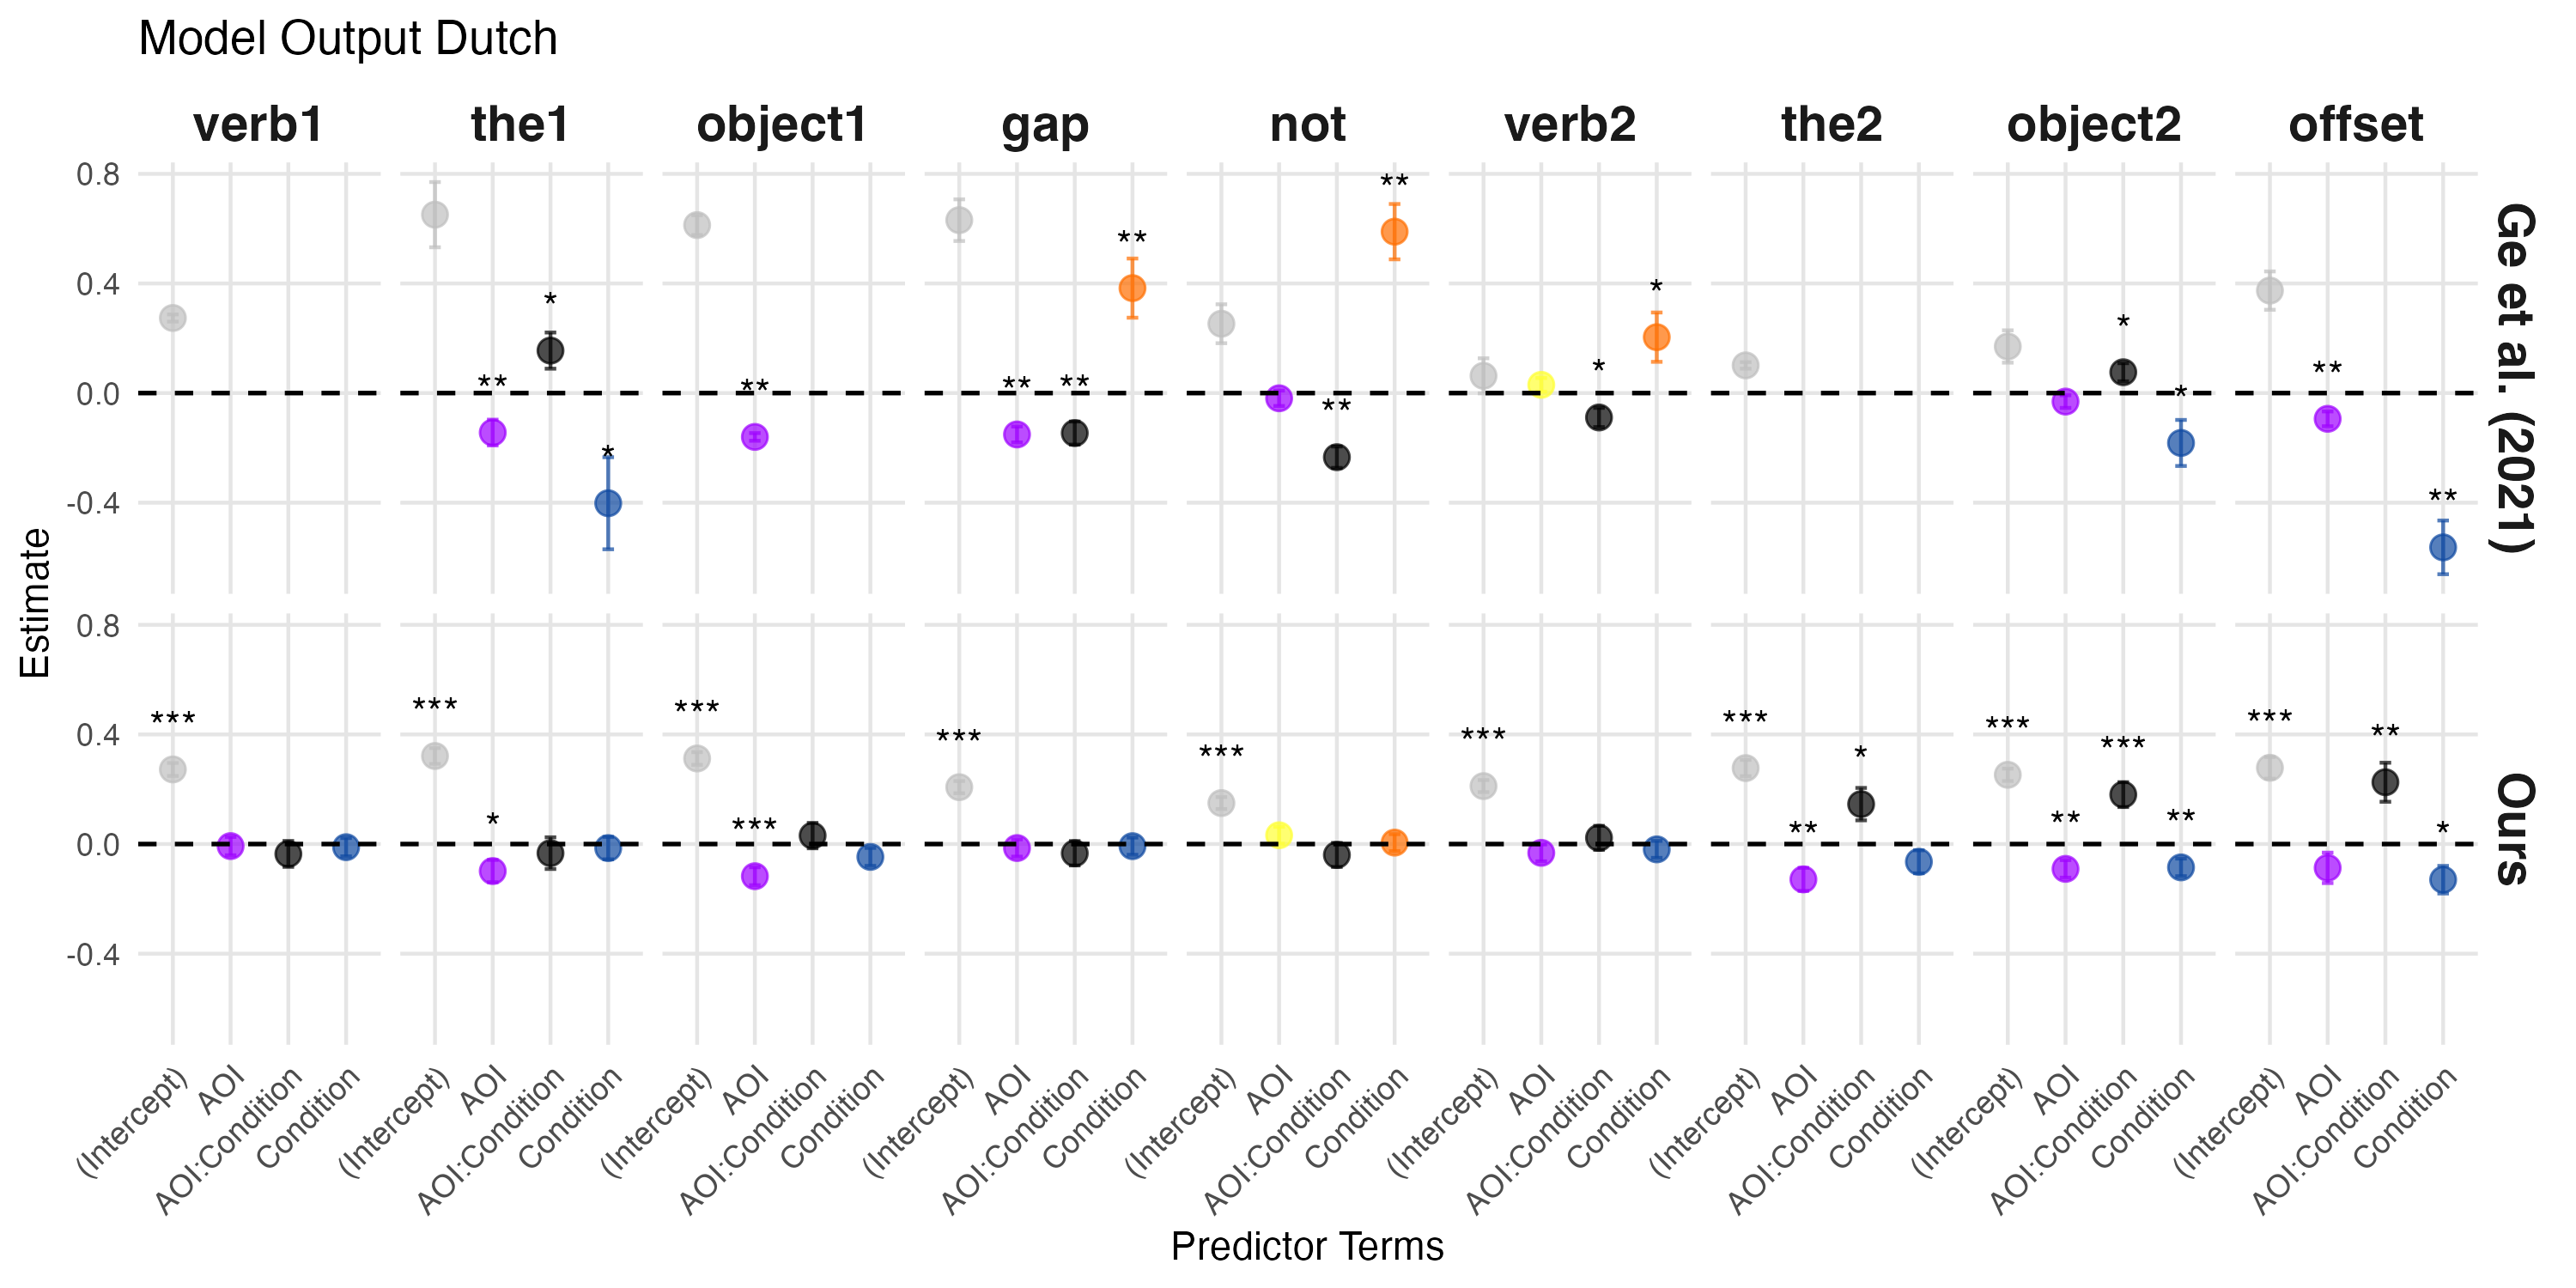
\includegraphics[width=\textwidth,height=\textheight,keepaspectratio]{viz/model_plot_dutch.png}
    \caption{Model outputs for L1 Dutch-L2 English participants across nine modeled time bins. Order of time bins appears in order across the top. Estimates of \cite{Ge2021} data appears on top while our data appears below. Significance levels 0.05, 0.01, and 0.001 are indicated by *, **, and ***, respectively above the estimate.}
    \label{fig:model_plot_dutch}
\end{figure}





\subsubsection{Methodological refinement: A ``focused" approach}

Whereas fidelity in replication is essential, it is also necessary to evaluate whether the original analytical choices align with current best practices. The refinement phase of our analysis serves to enhance statistical rigor by addressing potential limitations such as model specification, overfitting, multiple comparisons, and analytical transparency.

Here, we implement refined statistical approaches that maintain the interpretability of the original findings while increasing statistical robustness. This includes evaluating model assumptions, testing alternative specifications that account for variance more effectively, and applying more conservative corrections to reduce the likelihood of Type I errors. By implementing these refinements, we ensure that our results reflect patterns in the data, rather than artifacts of less stringent analytical choices.

These refinements do not alter the core structure of the replication but rather provide a more precise and statistically rigorous evaluation of the original claims. By comparing our refined results to both the original and replicated findings, we can assess whether methodological improvements impact the observed effects and whether the key conclusions of \cite{Ge2021} remain stable across different analytical approaches.

The first refinement we make is analyzing both binary competitor fixations and target fixations separately, rather than relying on aggregated measures. This approach provides a more comprehensive view of participants’ behavior, capturing differences in how they allocate visual attention. Moreover, there is no theoretical justification for modeling an aggregate measure when fixation data itself (i.e., looking or not looking) is directly available. Secondly, we combine the analysis from both language groups to be able to compare both within language by condition and across participant L1. Fig \ref{fig:english_fix2} shows a more interpretable version of Figure \ref{fig:english_fix}, which allows the reader to compare when fixations to specific AOI deviate from each other and not just across conditions.

\begin{figure}[H]  % 'p' puts it on its own page
    \centering
    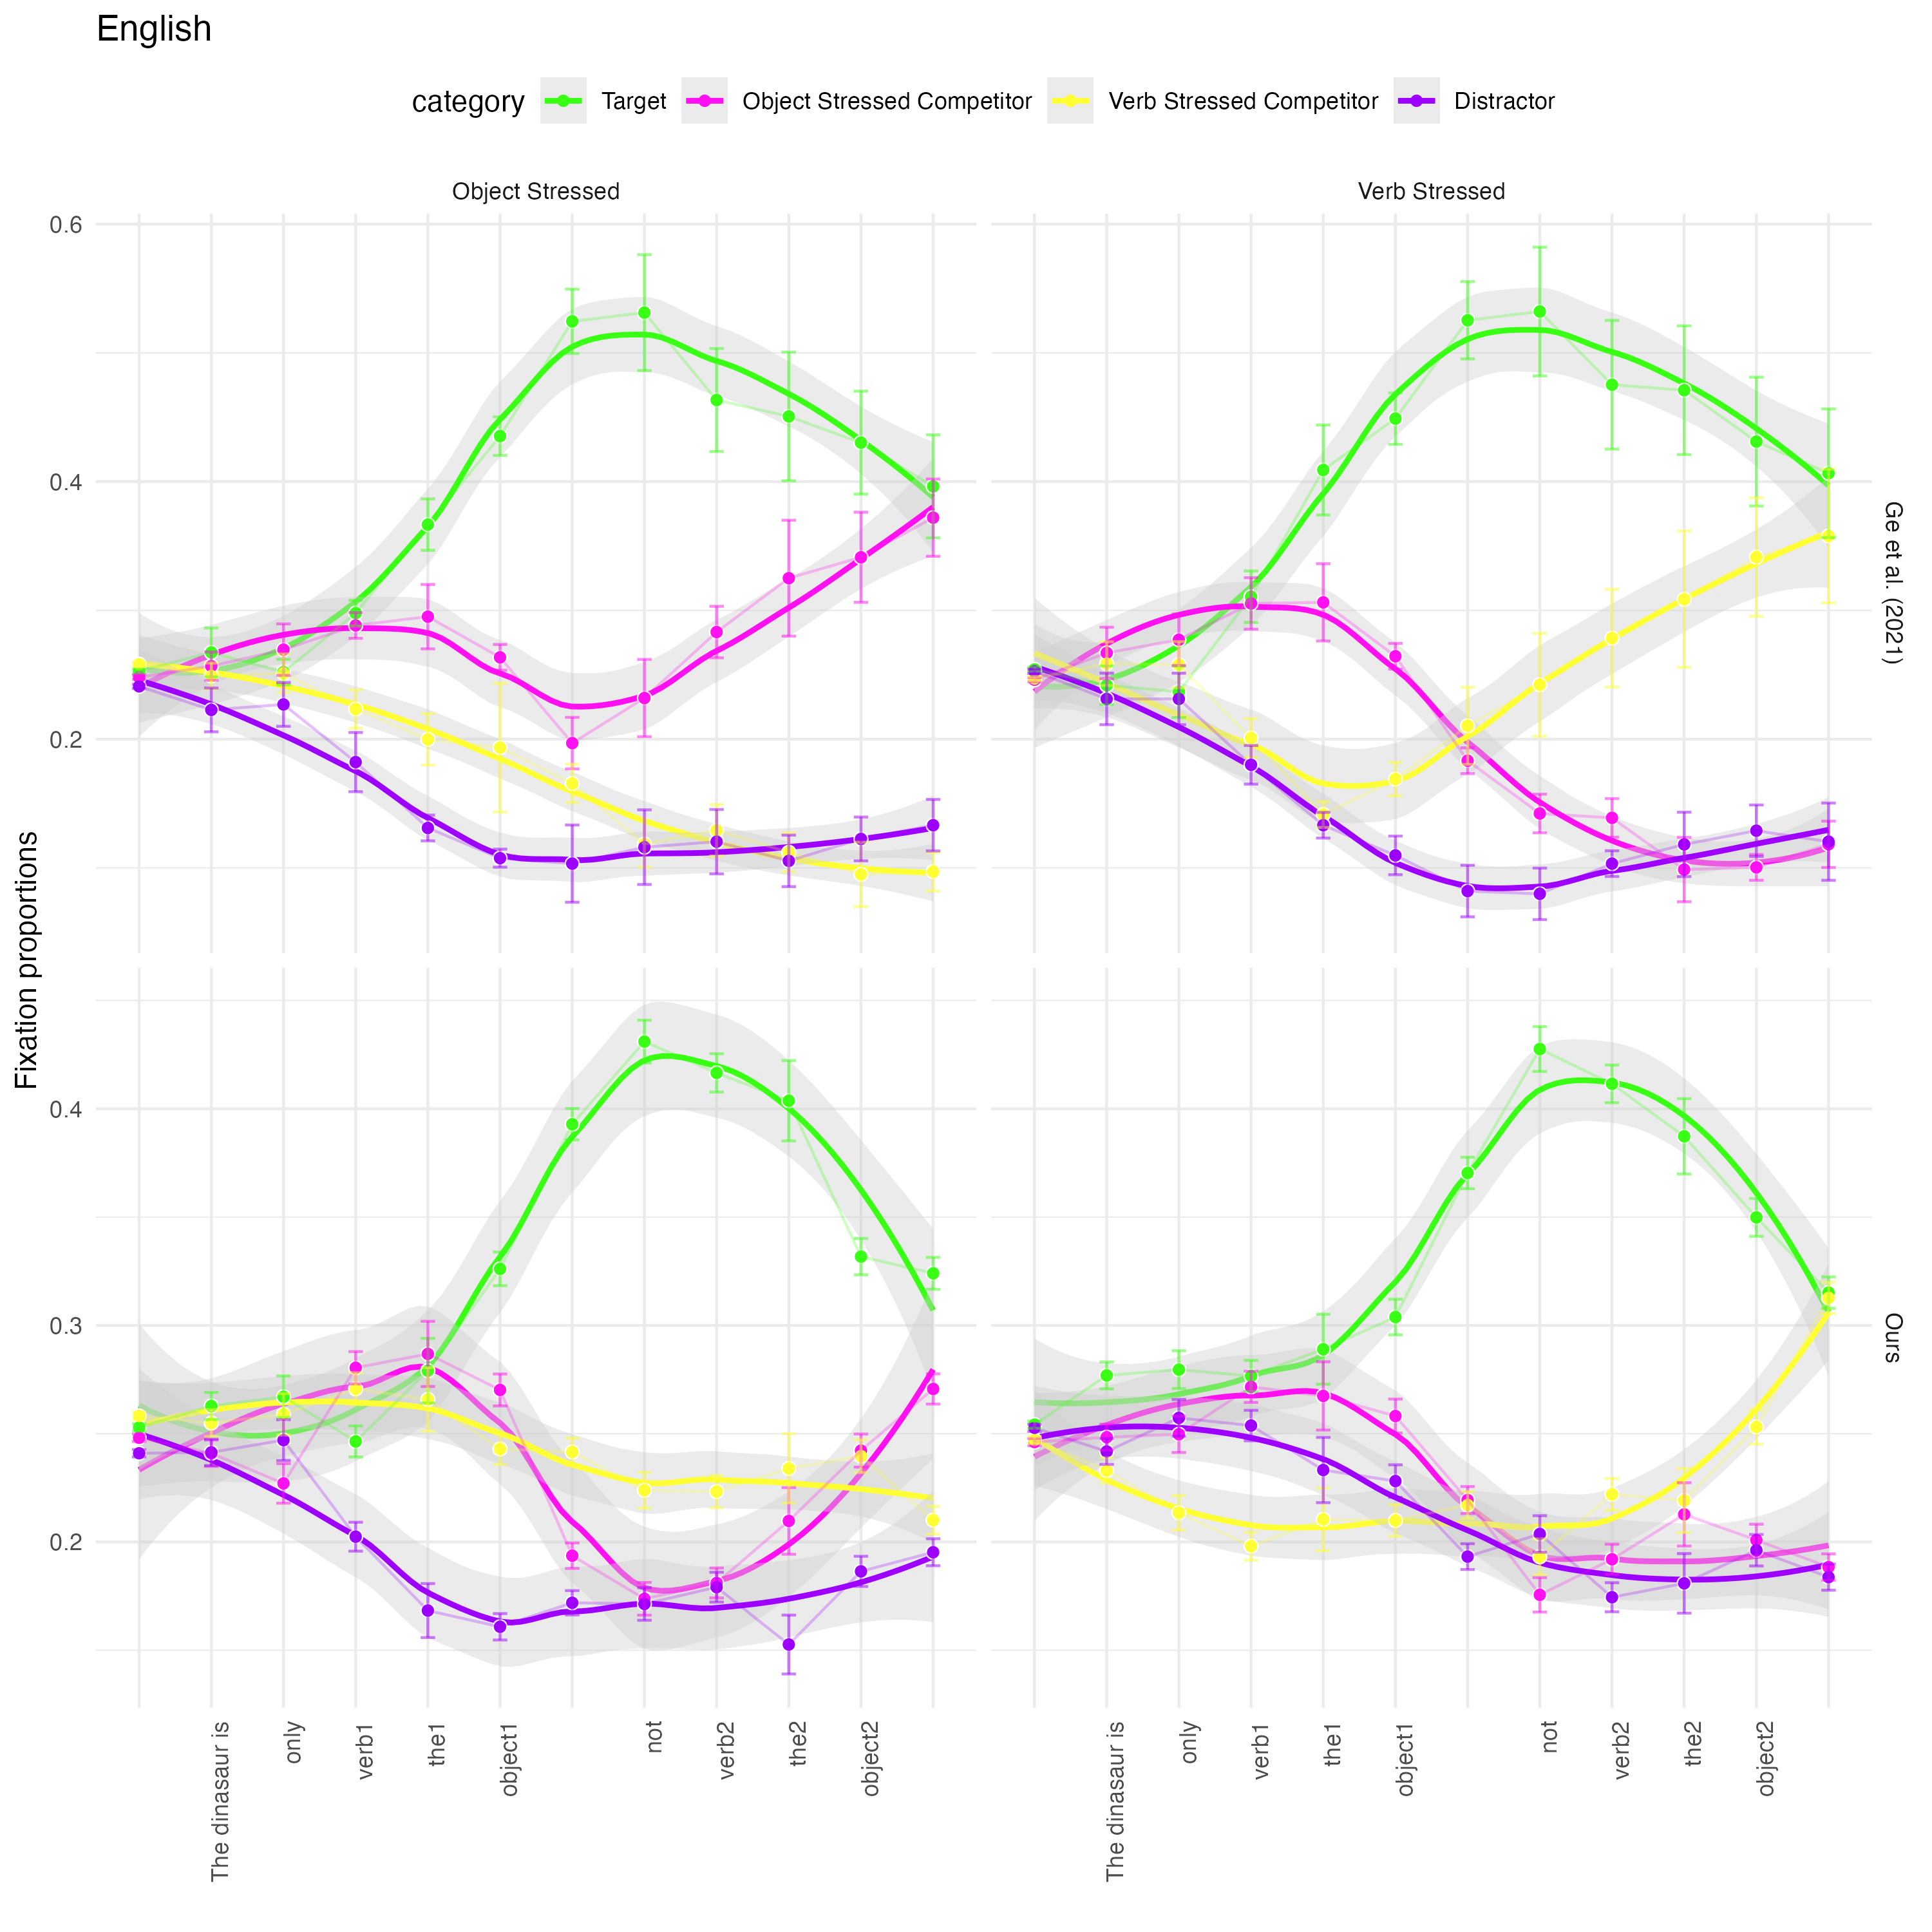
\includegraphics[width=\textwidth,height=\textheight,keepaspectratio]{viz/english_fix2.png}
    \caption{fixation proportions for English participants across object stressed (left) and verb stressed (right) sentences. Estimates of \citep{Ge2021} data appears on top while Our data appears below}
    \label{fig:english_fix2}
\end{figure}

For these refined models, we present both target models and competitor models. That is, we are comparing the target fixations (green lines in Figures \ref{fig:english_fix2} and \ref{fig:dutch_fix2}) in the target model and we are comparing the object competitor fixations (yellow lines in figures \ref{fig:english_fix2} and \ref{fig:dutch_fix2}) in the object focused sentences (left plots of figures \ref{fig:english_fix2} and \ref{fig:dutch_fix2}) as well as the verb competitor fixations (purple lines in figures \ref{fig:english_fix2} and \ref{fig:dutch_fix2}) during verb focused sentences (right plots of figures \ref{fig:english_fix2} and \ref{fig:dutch_fix2}) for the competitor models. 

\begin{figure}[H]  % 'p' puts it on its own page
    \centering
    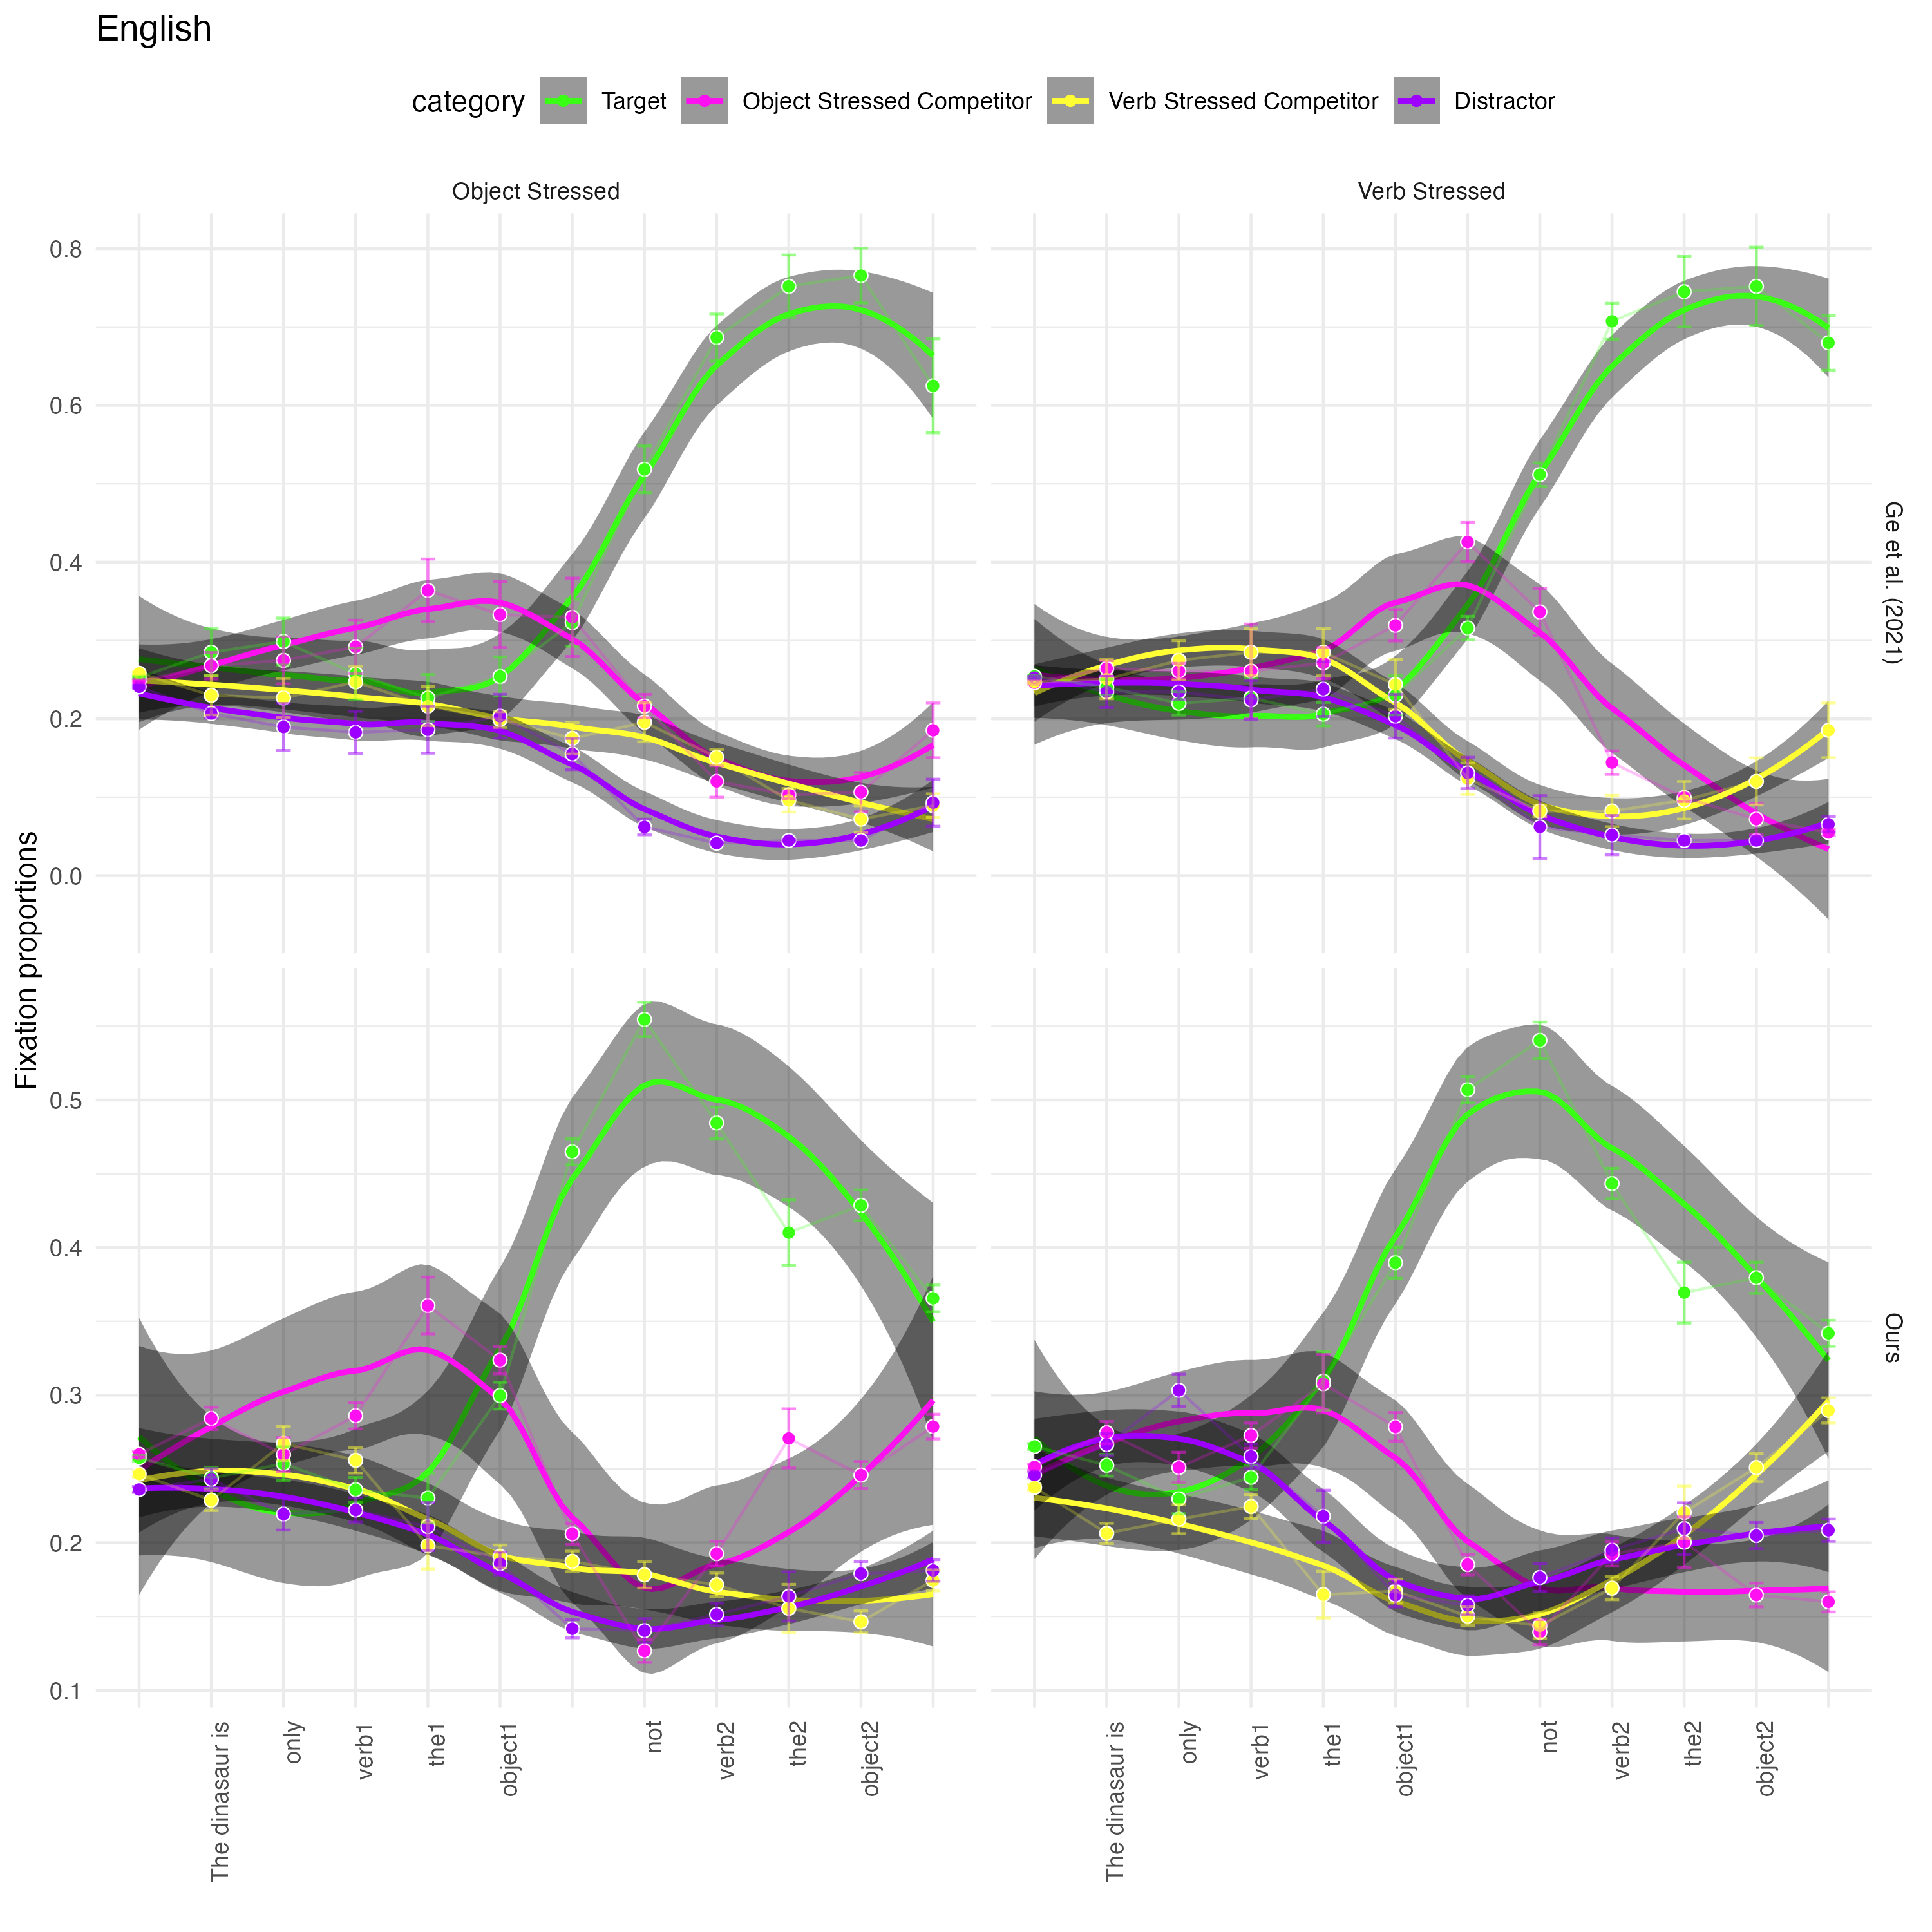
\includegraphics[width=\textwidth,height=\textheight,keepaspectratio]{viz/dutch_fix2.png}
    \caption{Fixation proportions for Dutch participants across object stressed (left) and verb stressed (right) sentences. Estimates of \cite{Ge2021} data appears on top while Our data appears below}
    \label{fig:dutch_fix2}
\end{figure}

An additional difference in our refined model is that we do all time bins in a single model. However, we split the sentence at the gap between the first phrase(e.g., ``the rabbit only verb1 the1 object1) and second phrase (e.g., ``not verb2 the2 object2). 

Unlike the linear mixed-effects models (LMMs) used in the fidelity modeling, this stage applies Generalized Additive Models (GAMs) to better capture time-dependent changes in fixation proportions. Since eye-tracking data unfolds continuously over time, GAMs provide a more flexible way to model the nonlinear dynamics of fixations that may not be well captured by traditional LMMs. In this approach, we compare two GAM variants: a full interaction model, which includes a three-way interaction between time, experiment group, and condition, and a main effects model, which assumes that changes in fixation proportions follow an additive pattern without time-dependent interactions. Both models include random smooth effects for participants, allowing for individual variability while capturing group-level fixation trends. Max models started with random items as well but none converged.

To determine the best-fitting model, we use BIC, where lower values indicate a better model fit. Unlike LMMs, which assume linear relationships between predictors and fixation proportions, GAMs allow for smooth, nonlinear changes over time, making them particularly well-suited for tracking how fixations dynamically evolve in response to prosodic cues. By using GAMs, we ensure that our analysis captures fine-grained temporal patterns in visual attention that might be overlooked by standard mixed-effects models.

Results of our 4 models (target-competitor models and phrase 1-phrase 2) are as follows. For the first phrase of the target models, a positive main effect stress was found ($\beta$ = 0.155, \textit{SE} = 0.053, \textit{t} = 2.93, \textit{p} = 0.003), indicating more target fixations during object focus sentences. A positive main effect of time ($\beta$ = 0.067, \textit{SE} = 0.012, \textit{t} = 5.66, \textit{p} $<$ 0.001)
 indicates increased looks to targets over the first phrase in general. In terms of interactions, a negative interaction between L1 and stress was found ($\beta$ = -0.316, \textit{SE} = 0.084, \textit{t} = -3.76, \textit{p} $<$ 0.001), indicating less looks during verb stressed stimuli for English participants. Also, we found a negative interaction between time and stress in phrase 1 of the target model ($\beta$ = -0.036, \textit{SE} = 0.017, \textit{t} = -2.12, \textit{p} = 0.034), indicating more verb looks to targets later on in phrase one for verb focused sentences. Lastly, the positive three way interaction between time, L1, and stress ($\beta$ = 0.136, \textit{SE} = 0.027, \textit{t} = 5.12, \textit{p} $<$ 0.001) indicates that over time, English participants exhibited an increasing trend in fixations to the target in verb-stressed sentences, in contrast to Dutch participants.
 
 For target fixations during the second phrase, a main effect of L1 ($\beta$ = 0.834, \textit{SE} = 0.237, \textit{t} = 3.52, \textit{p} $<$ 0.001) indicates that English speakers had significantly more looks to targets during the second phrase. Additionally, the negative main effect of time ($\beta$ = -0.137, \textit{SE} = 0.012, \textit{t} = -11.36, \textit{p} $<$ .001) indicates less looks to targets over the second phrase. The negative interaction between L1 and time ($\beta$ = -0.058, \textit{SE} = 0.019, \textit{t} = -3.09, \textit{p} = 0.002) indicates more looks to targets for Dutch L1 participants over time.

For the competitor model first phrase model, a positive main effect of time was found ($\beta$ = 0.056, \textit{SE} = 0.012, \textit{t} = 4.63, \textit{p} $<$ 0.001) indicating more looks to competitors over time during the first phrase. The negative interaction between time and stress was found ($\beta$ = -0.095, \textit{SE} = 0.018, \textit{t} = -5.26, \textit{p} $<$ 0.001), indicating more looks to verb competitors as time increases. No significant effects were found for the second phrase competitor model. Lastly, the negative interaction between L1 and stress ($\beta$ = -0.178, \textit{SE} = 0.086, \textit{t} = -2.06, \textit{p} = 0.040) indicates more looks to verb competitor for Dutch participants.

For the second phrase competitor model, a main positive effect of time was found ($\beta$ = 0.161, \textit{SE} = 0.014, \textit{t} = 11.42, \textit{p} $<$ 0.001), indicating that more looks to competitors occurred over the duration of the second phrase. The positive interaction between time and L1 ($\beta$ = 0.055, \textit{SE} = 0.022, \textit{t} = 2.50, \textit{p} = 0.012) indicates that Dutch speakers looked to competitors more as time went on over the second phrase. 

\begin{figure}[H]  % 'p' puts it on its own page
    \centering
    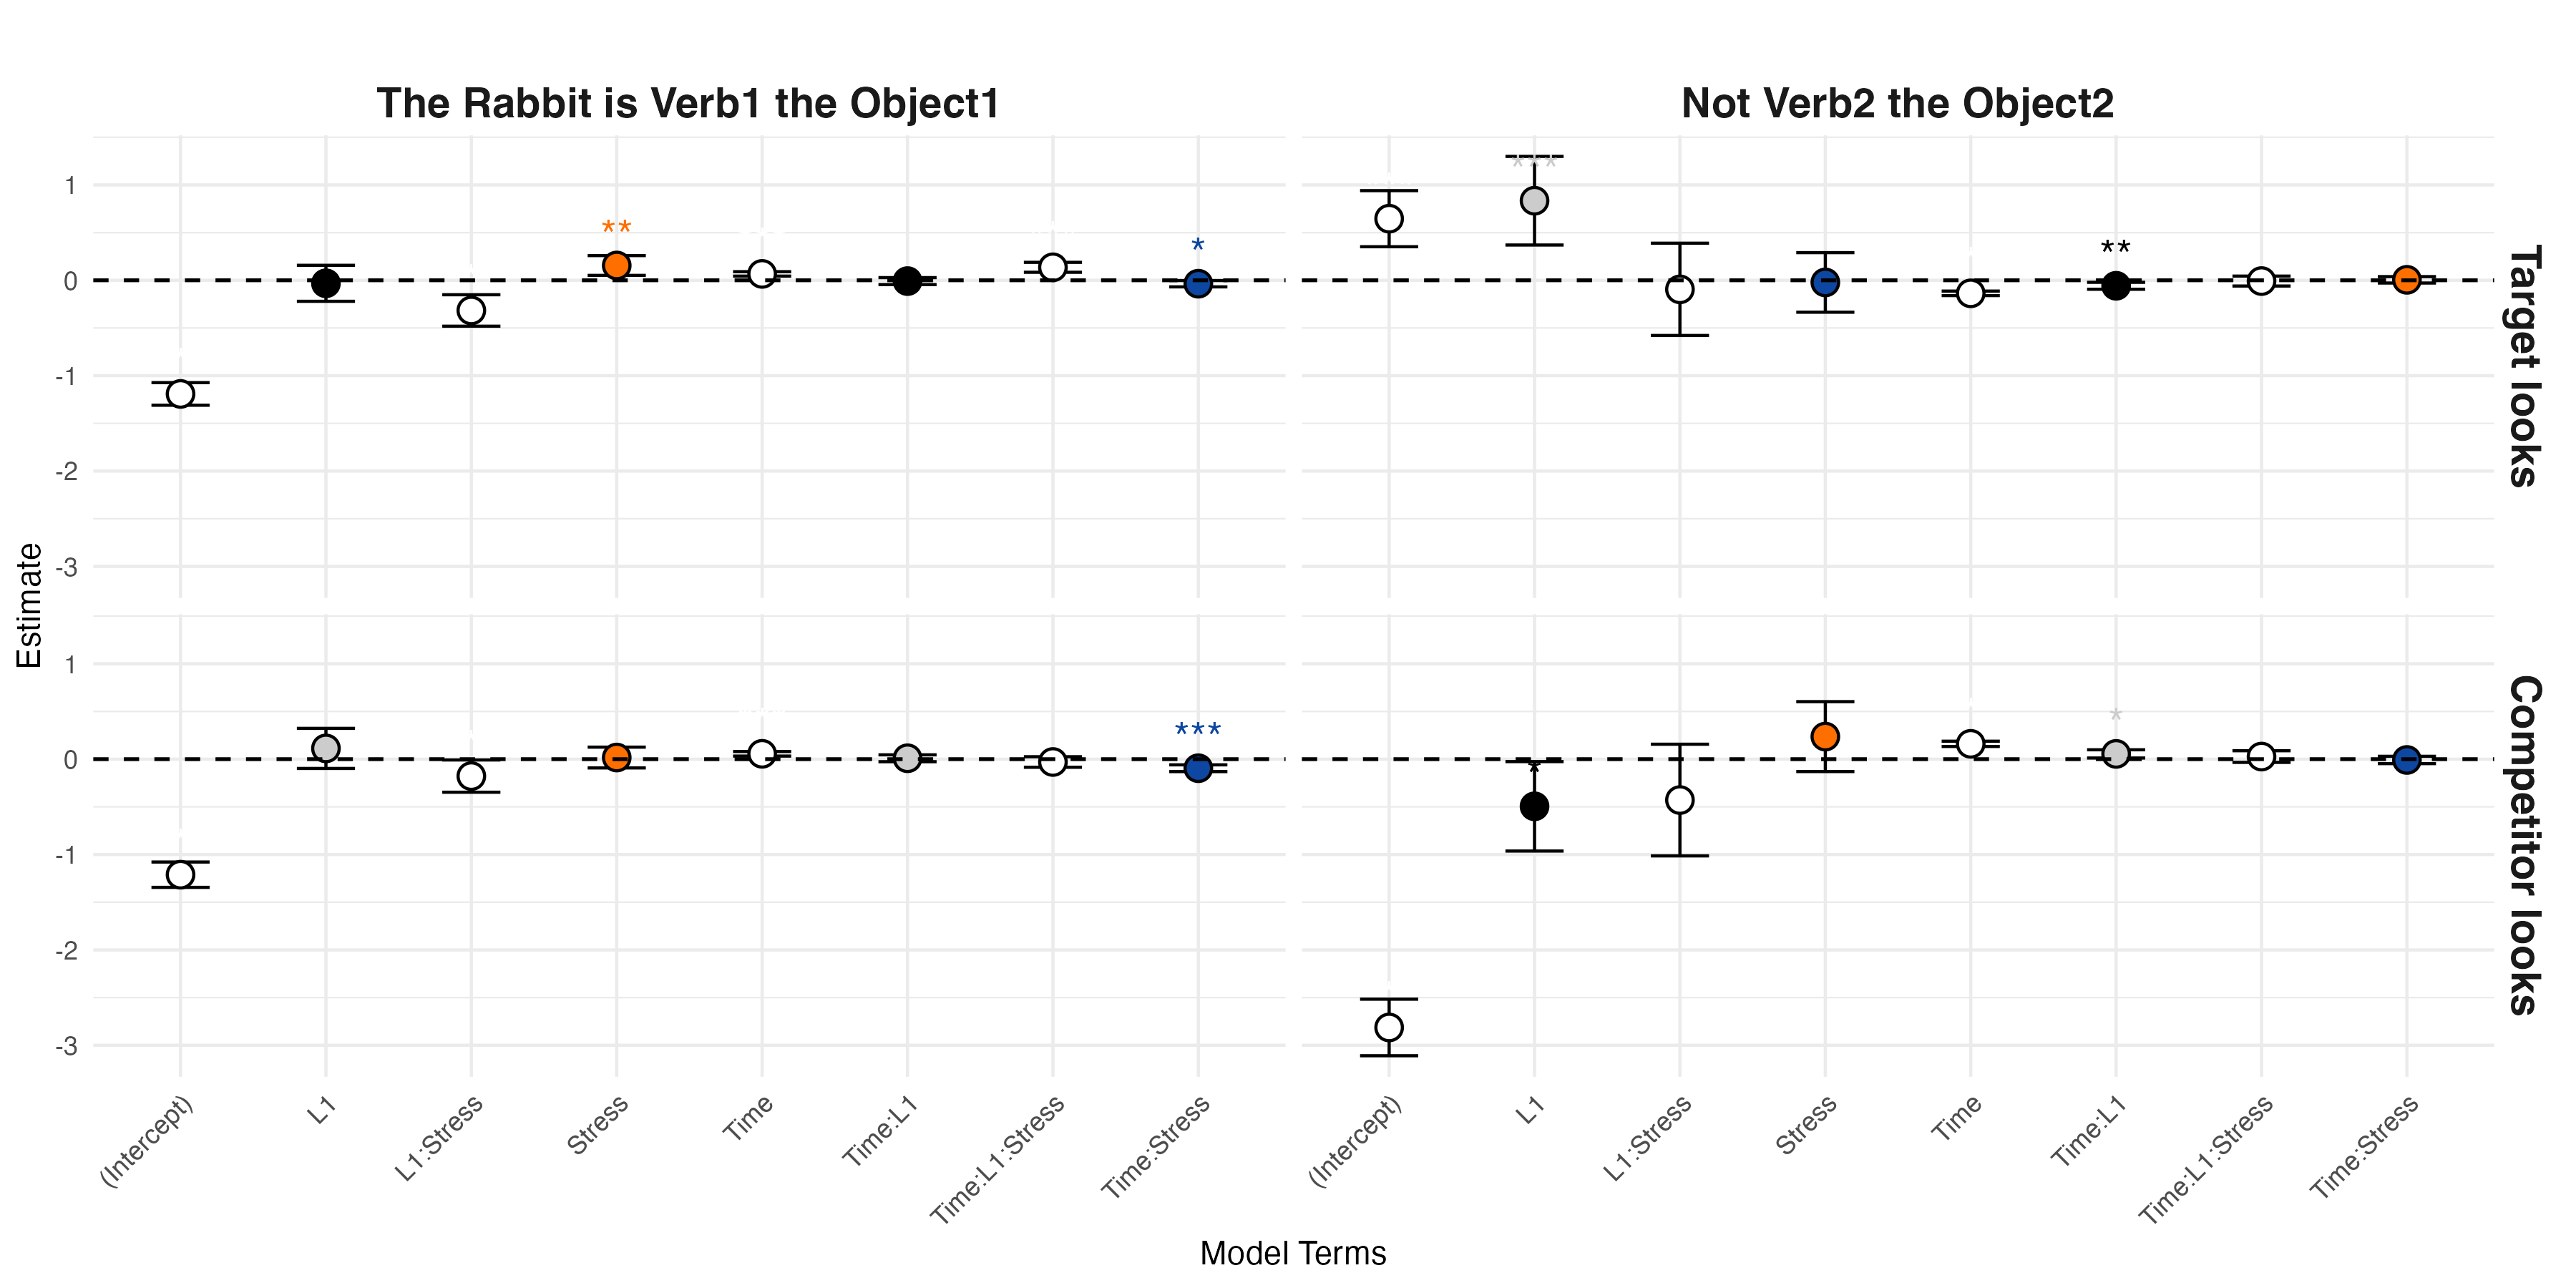
\includegraphics[width=\textwidth,height=\textheight,keepaspectratio]{viz/gam_mod_out.png}
    \caption{things}
    \label{fig:gam_mod_out}
\end{figure}

\subsection{Extension}

Beyond replication and refinement, we extend the analysis to explore additional theoretical questions not examined in \cite{Ge2021}. Specifically, we ask whether the observed differences in focus processing reflect a fundamental processing distinction or whether they can be attributed to individual differences among participants, irrespective of L1. Additionally, we investigate whether fixations to a particular target or competitor are systematically influenced by fine-grained acoustic-phonetic properties of the stimuli, moving beyond aggregated data to better capture how specific speech input characteristics shape perceptual adaptation \citep{xie2023adaptive}.

While the original study provided valuable insights into focus processing, it did not explicitly examine the role of individual cognitive and perceptual differences in shaping listener behavior. Given prior research suggesting that factors such as working memory, auditory perception, and cognitive control contribute to variability in language processing, we test whether these factors modulate eye-movement patterns in response to focus cues. By integrating individual difference measures with detailed stimulus-level analyses, we follow recommendations from \cite{xie2023adaptive} to more precisely map how perception adapts to variation in the speech signal. Individual differences among our participants are visualized in Figure \ref{fig:combined_plot}, which presents a comprehensive view of the multidimensional nature of these differences. 

\clearpage
\begin{figure}[H]  % 'p' puts it on its own page
    \centering
    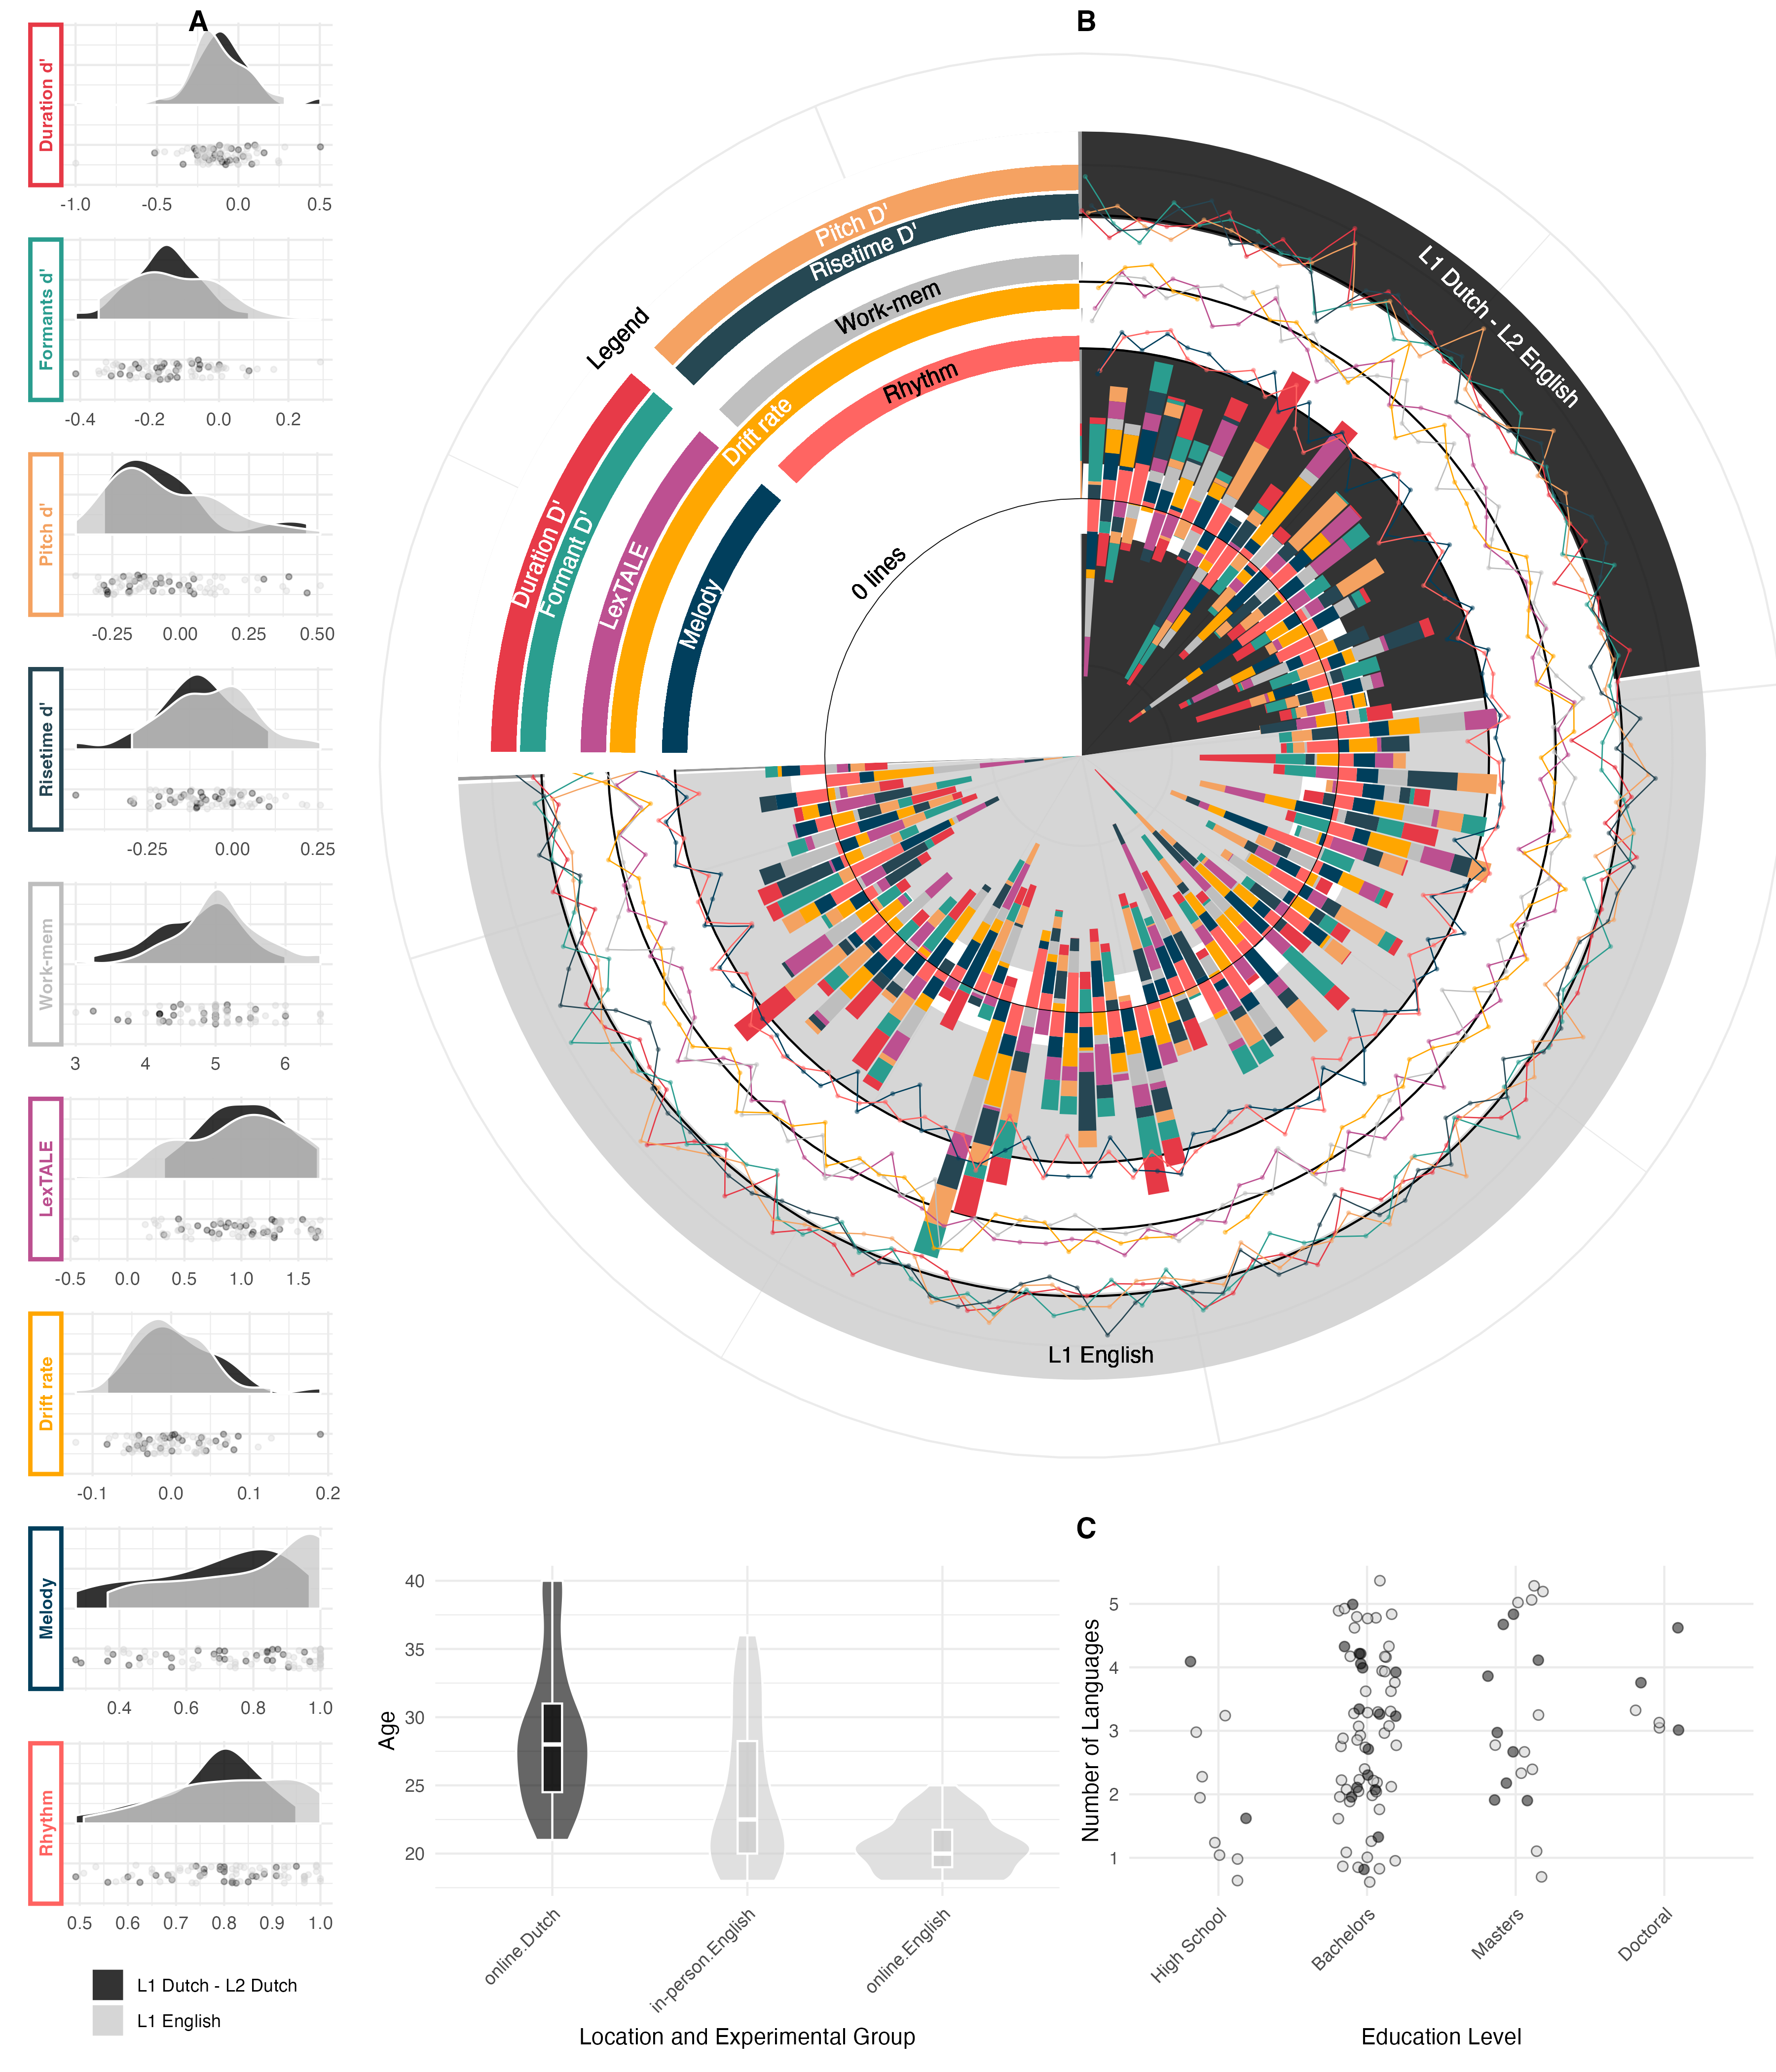
\includegraphics[width=\textwidth,height=\textheight,keepaspectratio]{viz/combined_plot_circle.png}
    \caption{describe what is going on here- A- tasks across the Dutch and English, B individual difference vectors for each participant, C background information on participants}
    \label{fig:combined_plot}
\end{figure}
\clearpage


To quantify the acoustic properties of the stimuli, we extracted key measures from the speech recordings using parselmouth \citep{Boersma2022} in Python, facilitated through the reticulate package \citep{Ushey2022} in R. First, TextGrid annotations were parsed to determine onset and offset times for each word, ensuring alignment between acoustic measures and eye-movement data. The stimuli were then segmented into time-aligned regions corresponding to critical sentence components (e.g., verb, object, focus phrases), allowing for a detailed examination of how fixations to targets and competitors correspond to systematic acoustic variation. The pitch of the stimuli by time bin are shown in fig \ref{fig:acoustic}.

\begin{figure}[H]  % 'p' puts it on its own page
    \centering
    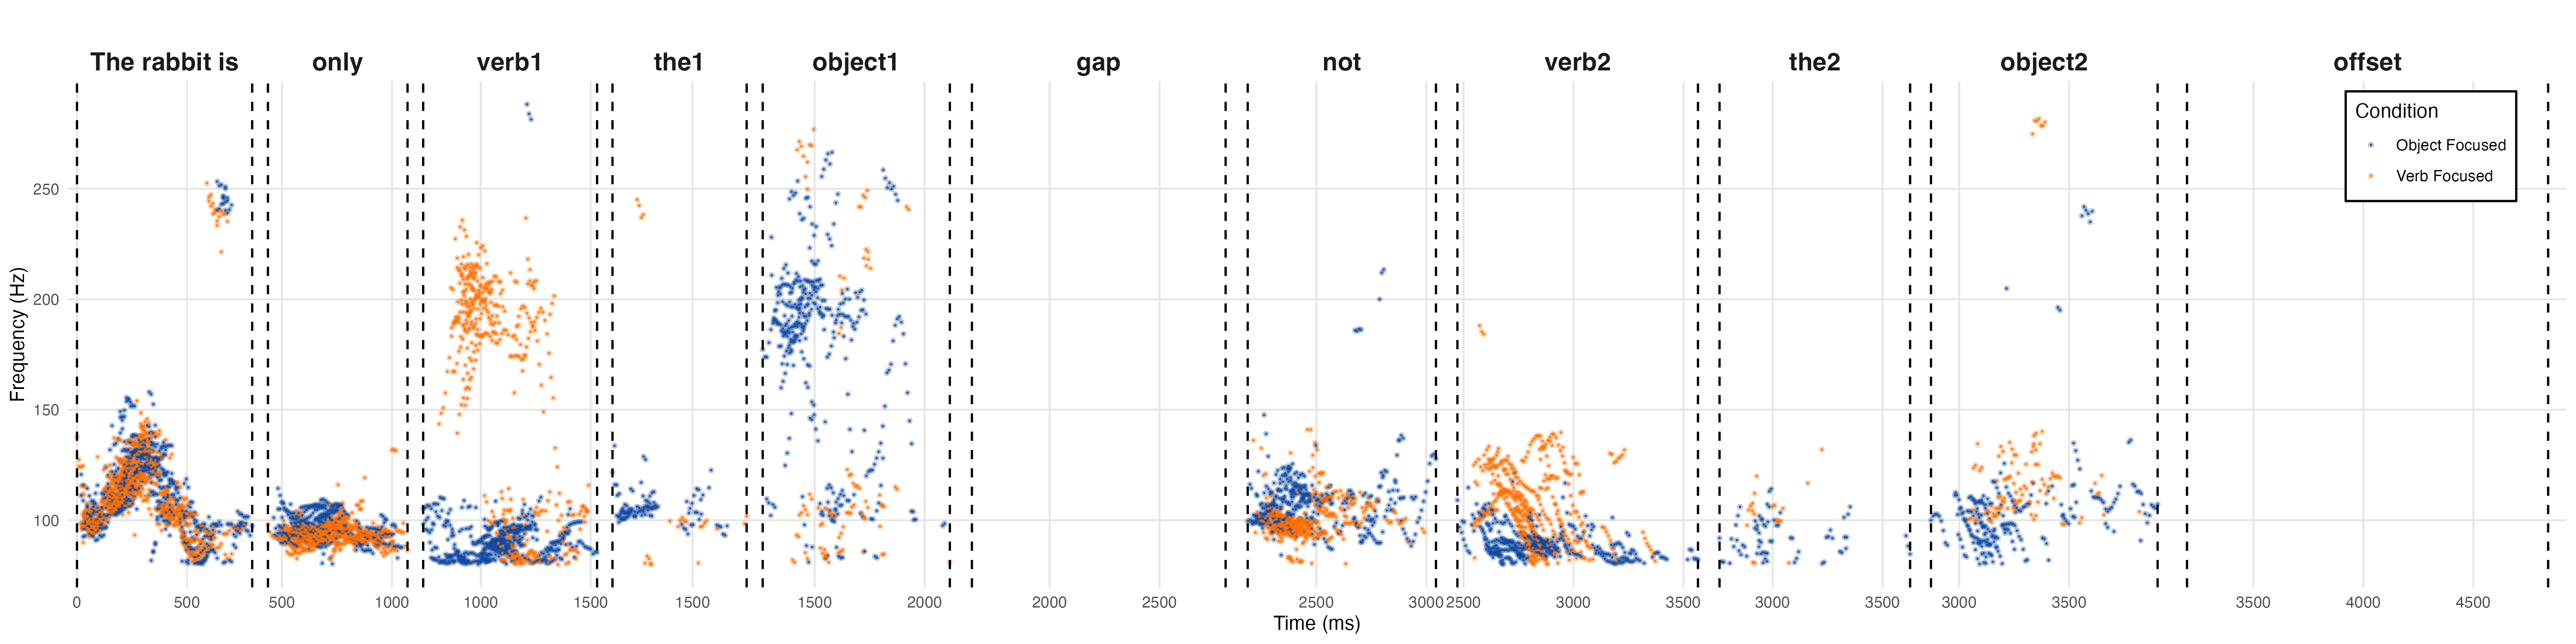
\includegraphics[width=\textwidth,height=\textheight,keepaspectratio]{viz/accoustic.png}
    \caption{things}
    \label{fig:acoustic}
\end{figure}

We computed scaled acoustic measures to normalize differences across stimuli, capturing four key parameters. Pitch range (min-max pitch per word) was extracted to track variations in fundamental frequency, reflecting tonal and prosodic changes. Stress prominence was measured in lower frequency bands, providing an indicator of emphasis within each stimulus. Amplitude, analyzed in db served as an energy-based measure of prominence, helping to assess variations in speech intensity. Finally, word duration was computed to account for differences in articulation time across conditions, ensuring that segmental timing effects were incorporated into our analysis. All scaled values can be seen in figure \ref{fig:acoustic_faceted}.

\begin{figure}[H]  % 'p' puts it on its own page
    \centering
    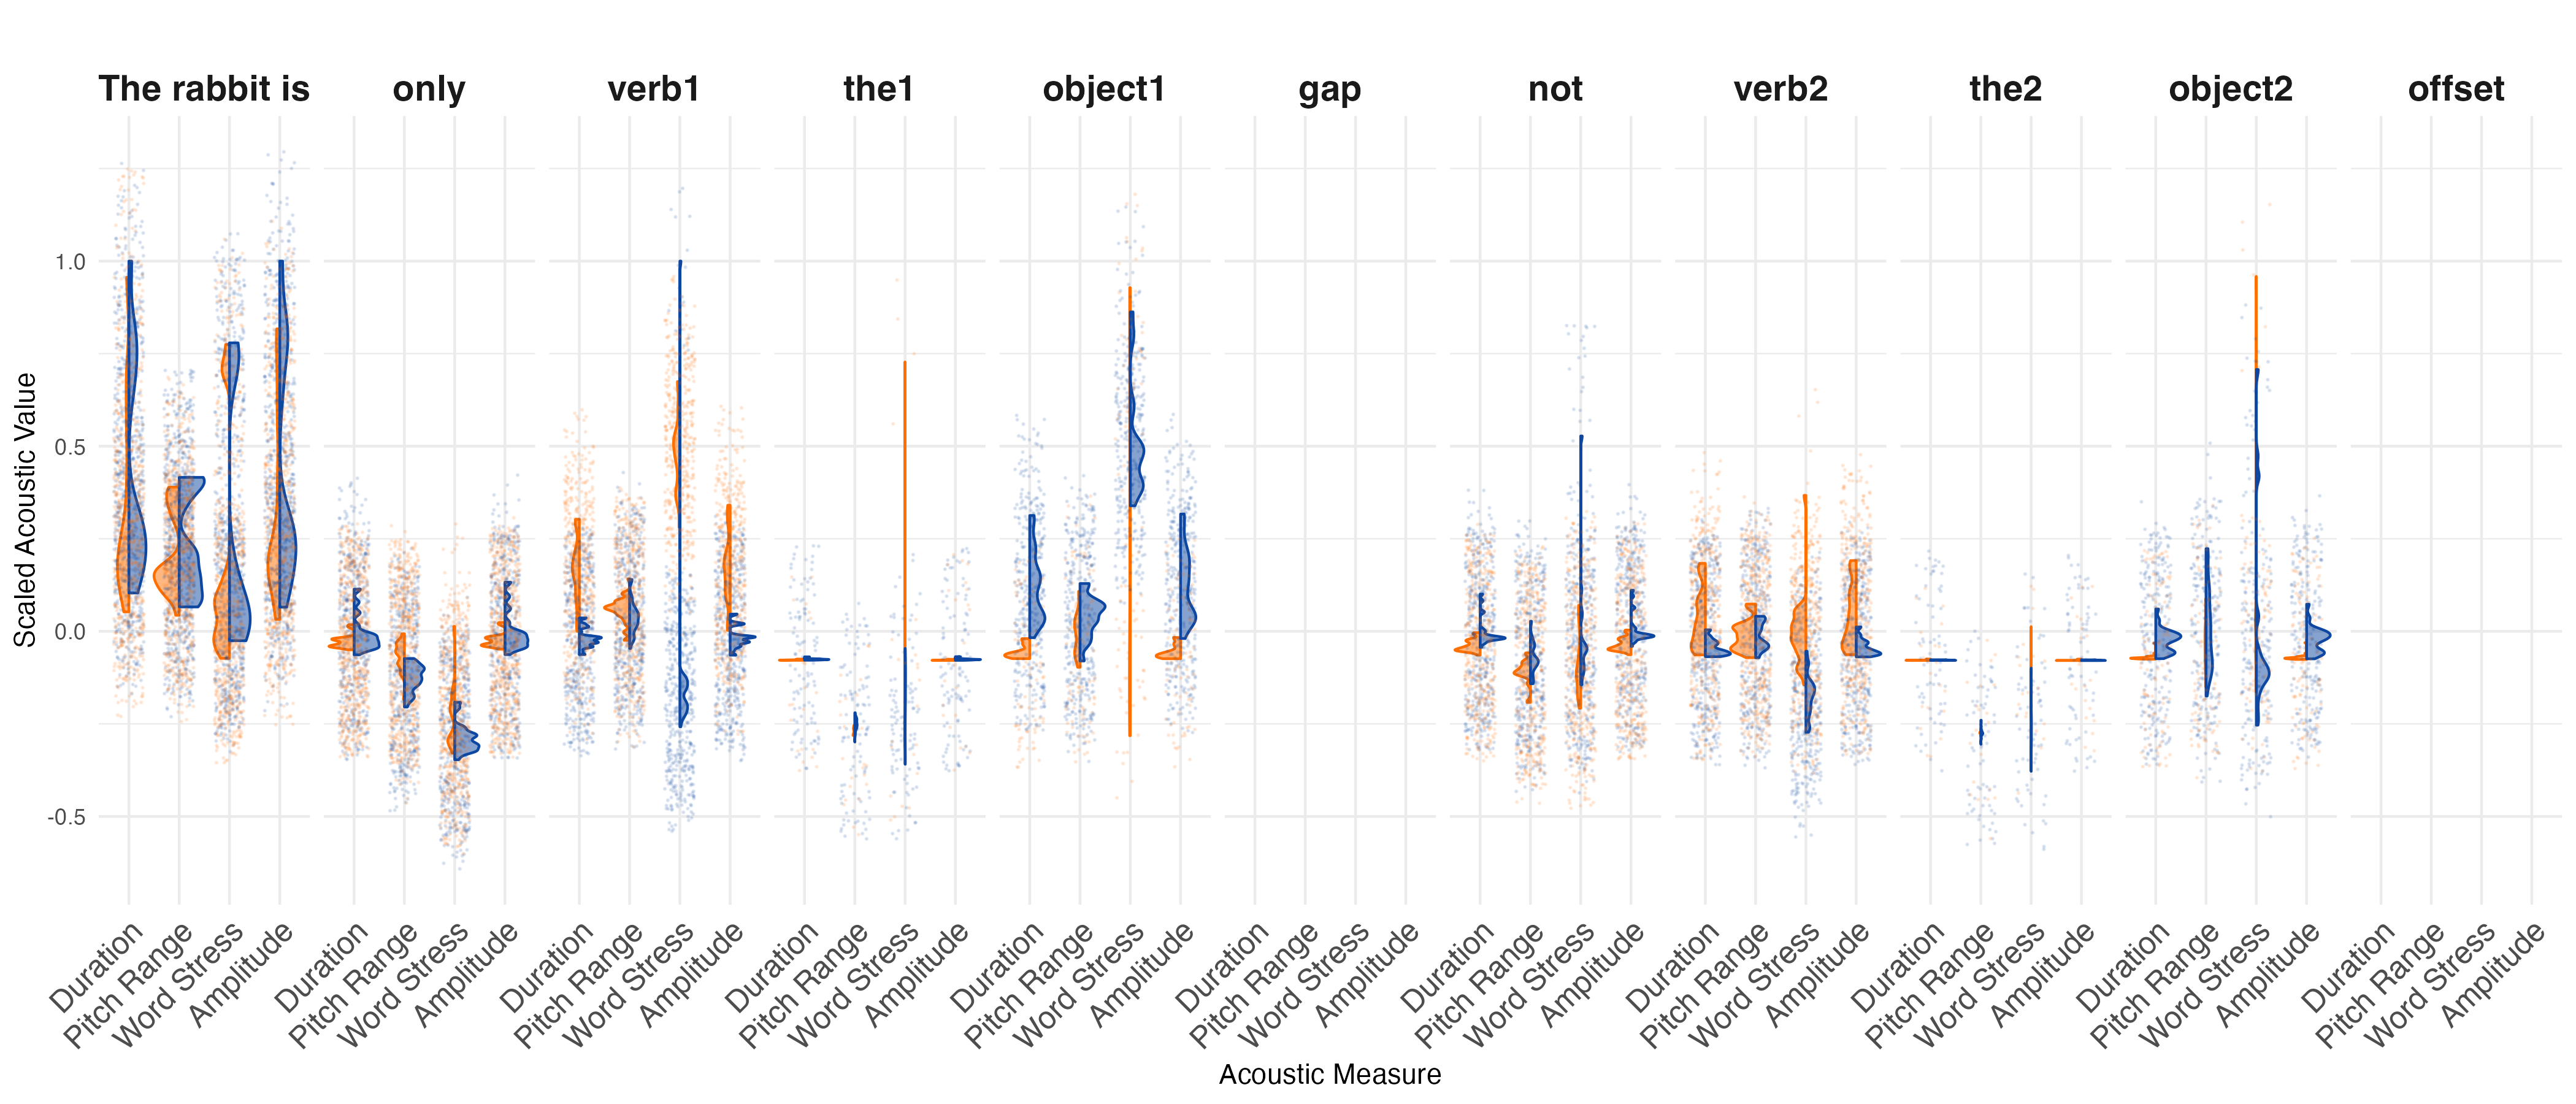
\includegraphics[width=\textwidth,height=\textheight,keepaspectratio]{viz/acoustic_faceted.png}
    \caption{things}
    \label{fig:acoustic_faceted}
\end{figure}


In terms of statistical analysis use the refined modeling approach as a baseline procedure. To optimize model selection while maintaining interpretability, we employed LASSO-GAM Feature Selection, combining LASSO regression (cv.glmnet(); \citep{Friedman2010} with Generalized Additive Models (GAMs) (mgcv; \citep{Wood2017}. First, LASSO identified the most predictive variables from a set of individual differences (e.g., cognitive abilities, auditory perception, lexical knowledge), acoustic features (e.g., pitch, duration, amplitude), and experimental conditions, while regularizing to prevent overfitting.

Next, the selected predictors were incorporated into a GAM to model nonlinear time effects and random participant variability. This data-driven approach ensures that only the most informative factors contribute to the model, balancing flexibility, interpretability, and predictive accuracy.

The LASSO was applied in a generalized linear model (GLM) with a binomial link function, where the design matrix included individual differences, acoustic properties, and experimental conditions, along with key interaction terms. The individual difference measures included working memory capacity, drift rate (decision-making efficiency), lexical knowledge (LexTALE score), and musical ability measures such as beat perception and melody discrimination. The acoustic features included pitch range (min-max pitch per word), duration, stress prominence (spectral tilt in lower frequencies), and amplitude (raw and dB-scaled). The experimental conditions included focus condition (object-focused vs. verb-focused) and participant group assignment (e.g., L1 background or training condition).

To account for potential interactive effects, we included key two-way and three-way interactions. These interactions tested whether perceptual, cognitive, and linguistic factors jointly influenced fixations. Specifically, we modeled interactions between individual differences and acoustic properties (e.g., pitch sensitivity × pitch range, beat perception × duration) and interactions between experimental conditions and perceptual abilities (e.g., focus condition × working memory, L1 background × stress prominence). Additionally, we included a three-way interaction to examine whether the effect of working memory on lexical processing varied as a function of drift rate and lexical knowledge.

Results from the modeling are presented next. Order will start with first phrase target fixation and make its way to second phrase competitor fixations. In the target model of phrase one no main effects were found. However, the interaction between duration d' and acoustic duration of the word ($\beta$ = -0.848, \textit{SE} = 0.205, \textit{t} = -4.14, \textit{p} $<$ 0.001) indicate that less target looks occurred for those with lesser duration sensitivity during stimuli that have lower duration. Similarly, the positive interaction between formant d$'$ and word stress ($\beta$ = 0.230, \textit{SE} = 0.106, \textit{t} = 2.16, \textit{p} = 0.031) indicates more target fixations for those with better formant sensitivity for words with higher word stress. lastly, the positive interaction between pitch d$'$ and pitch range ($\beta$ = 0.144, \textit{SE} = 0.068, \textit{t} = 2.11, \textit{p} = 0.035) indicates that more target fixations occurred for individuals with greater pitch sensitivity for word bins with a larger pitch range.

 For the second phrase target model, a negative main effect of duration ($\beta$ = -0.357, \textit{SE} = 0.093, \textit{t} = -3.85, \textit{p} = 0.0001) indicates that shorter word acoustics lead to less target fixations. The main negative effect of stress ($\beta$ = -0.060, \textit{SE} = 0.022, \textit{t} = -2.72, \textit{p} = 0.0066) indicates that verb focused sentences generally had less target fixations during the second phrase. For interactions, the negative interaction between duration d$'$ and word duration ($\beta$ = -0.396, \textit{SE} = 0.125, \textit{t} = -3.18, \textit{p} = 0.0015) leads to less target fixations during the second phrase. Finally, the negative interaction between pitch range and melody ($\beta$ = -0.487, \textit{SE} = 0.110, \textit{t} = -4.42, \textit{p} $<$ .00001) indicates that for those with lower melodic abilities during phrases with lower pitch less target fixations occur.

 For the first phrase competitor model, a main negative effect of duration ($\beta$ = -0.477, \textit{SE} = 0.195, \textit{t} = -2.45, \textit{p} = .014) indicates less looks to competitors for lower duration word bins. The positive L1 main effect ($\beta$ = 0.325, \textit{SE} = 0.120, \textit{t} = 2.71, \textit{p} = .007) indicates more looks to competitors during the first syllable for Dutch participants. Also the positive main effect of word stress ($\beta$ = 0.197, \textit{SE} = 0.097, \textit{t} = 2.03, \textit{p} = .042) indicates more competitor looks for words with higher word stress. In terms of interactions, the positive interaction between duration d$'$ and duration of the word ($\beta$ = 0.853, \textit{SE} = 0.216, \textit{t} = 3.96, \textit{p} $<$ .001) indicates more competitor looks when words have longer durations during the first phrase. The effect is mirrored in positive interaction between formant d$'$ and word stress ($\beta$ = 0.419, \textit{SE} = 0.116, \textit{t} = 3.61, \textit{p} $<$ .001), which indicates more competitor looks for those with greater formant sensitivity when words have high word stress. The positive interaction between melody and pitch range ($\beta$ = 0.239, \textit{SE} = 0.072, \textit{t} = 3.33, \textit{p} $<$ .001) further indicates that for participants with higher melodic abilities, words with greater pitch range lead to more competitor fixations during the first phrase. Finally, the negative interaction between stress and L1 ($\beta$ = -0.267, \textit{SE} = 0.047, \textit{t} = -5.64, \textit{p} $<$ .001) indicates less competitor fixations for English speakers during verb stressed first phrases.

Our last model is the second phrase competitor model, where a positive main effect of duration ($\beta$ = 0.362, \textit{SE} = 0.091, \textit{t} = 3.96, \textit{p} $<$ .001) was found, which indicates more competitor fixations for words with shorter duration during the second syllable. The negative main effect of pitch d$'$ ($\beta$ = -0.393, \textit{SE} = 0.194, \textit{t} = -2.03, \textit{p} = .043) indicates less competitor fixations for participants with lower pitch sensitivity. Likewise, the positive main effect of stress ($\beta$ = 0.355, \textit{SE} = 0.077, \textit{t} = 4.63, \textit{p} $<$ .001) indicates greater competitor fixations during the second syllable for object focused phrases. For interactions, a negative interaction between L1 and stress ($\beta$ = -0.188, \textit{SE} = 0.052, \textit{t} = -3.64, \textit{p} $<$ 0.001) indicate less competitor fixations for English speakers during verb focus sentences in the second phrase. Very last, the positive interaction between pitch d$'$ and pitch range ($\beta$ = 0.664, \textit{SE} = 0.131, \textit{t} = 5.07, \textit{p} $<$ 0.001) indicates more competitor looks when a participant has more pitch sensitivity and the word has higher pitch range. All results for extension analyses can be found in figure \ref{fig:id_gam_mod_out}.

\begin{figure}[H]  % 'p' puts it on its own page
    \centering
    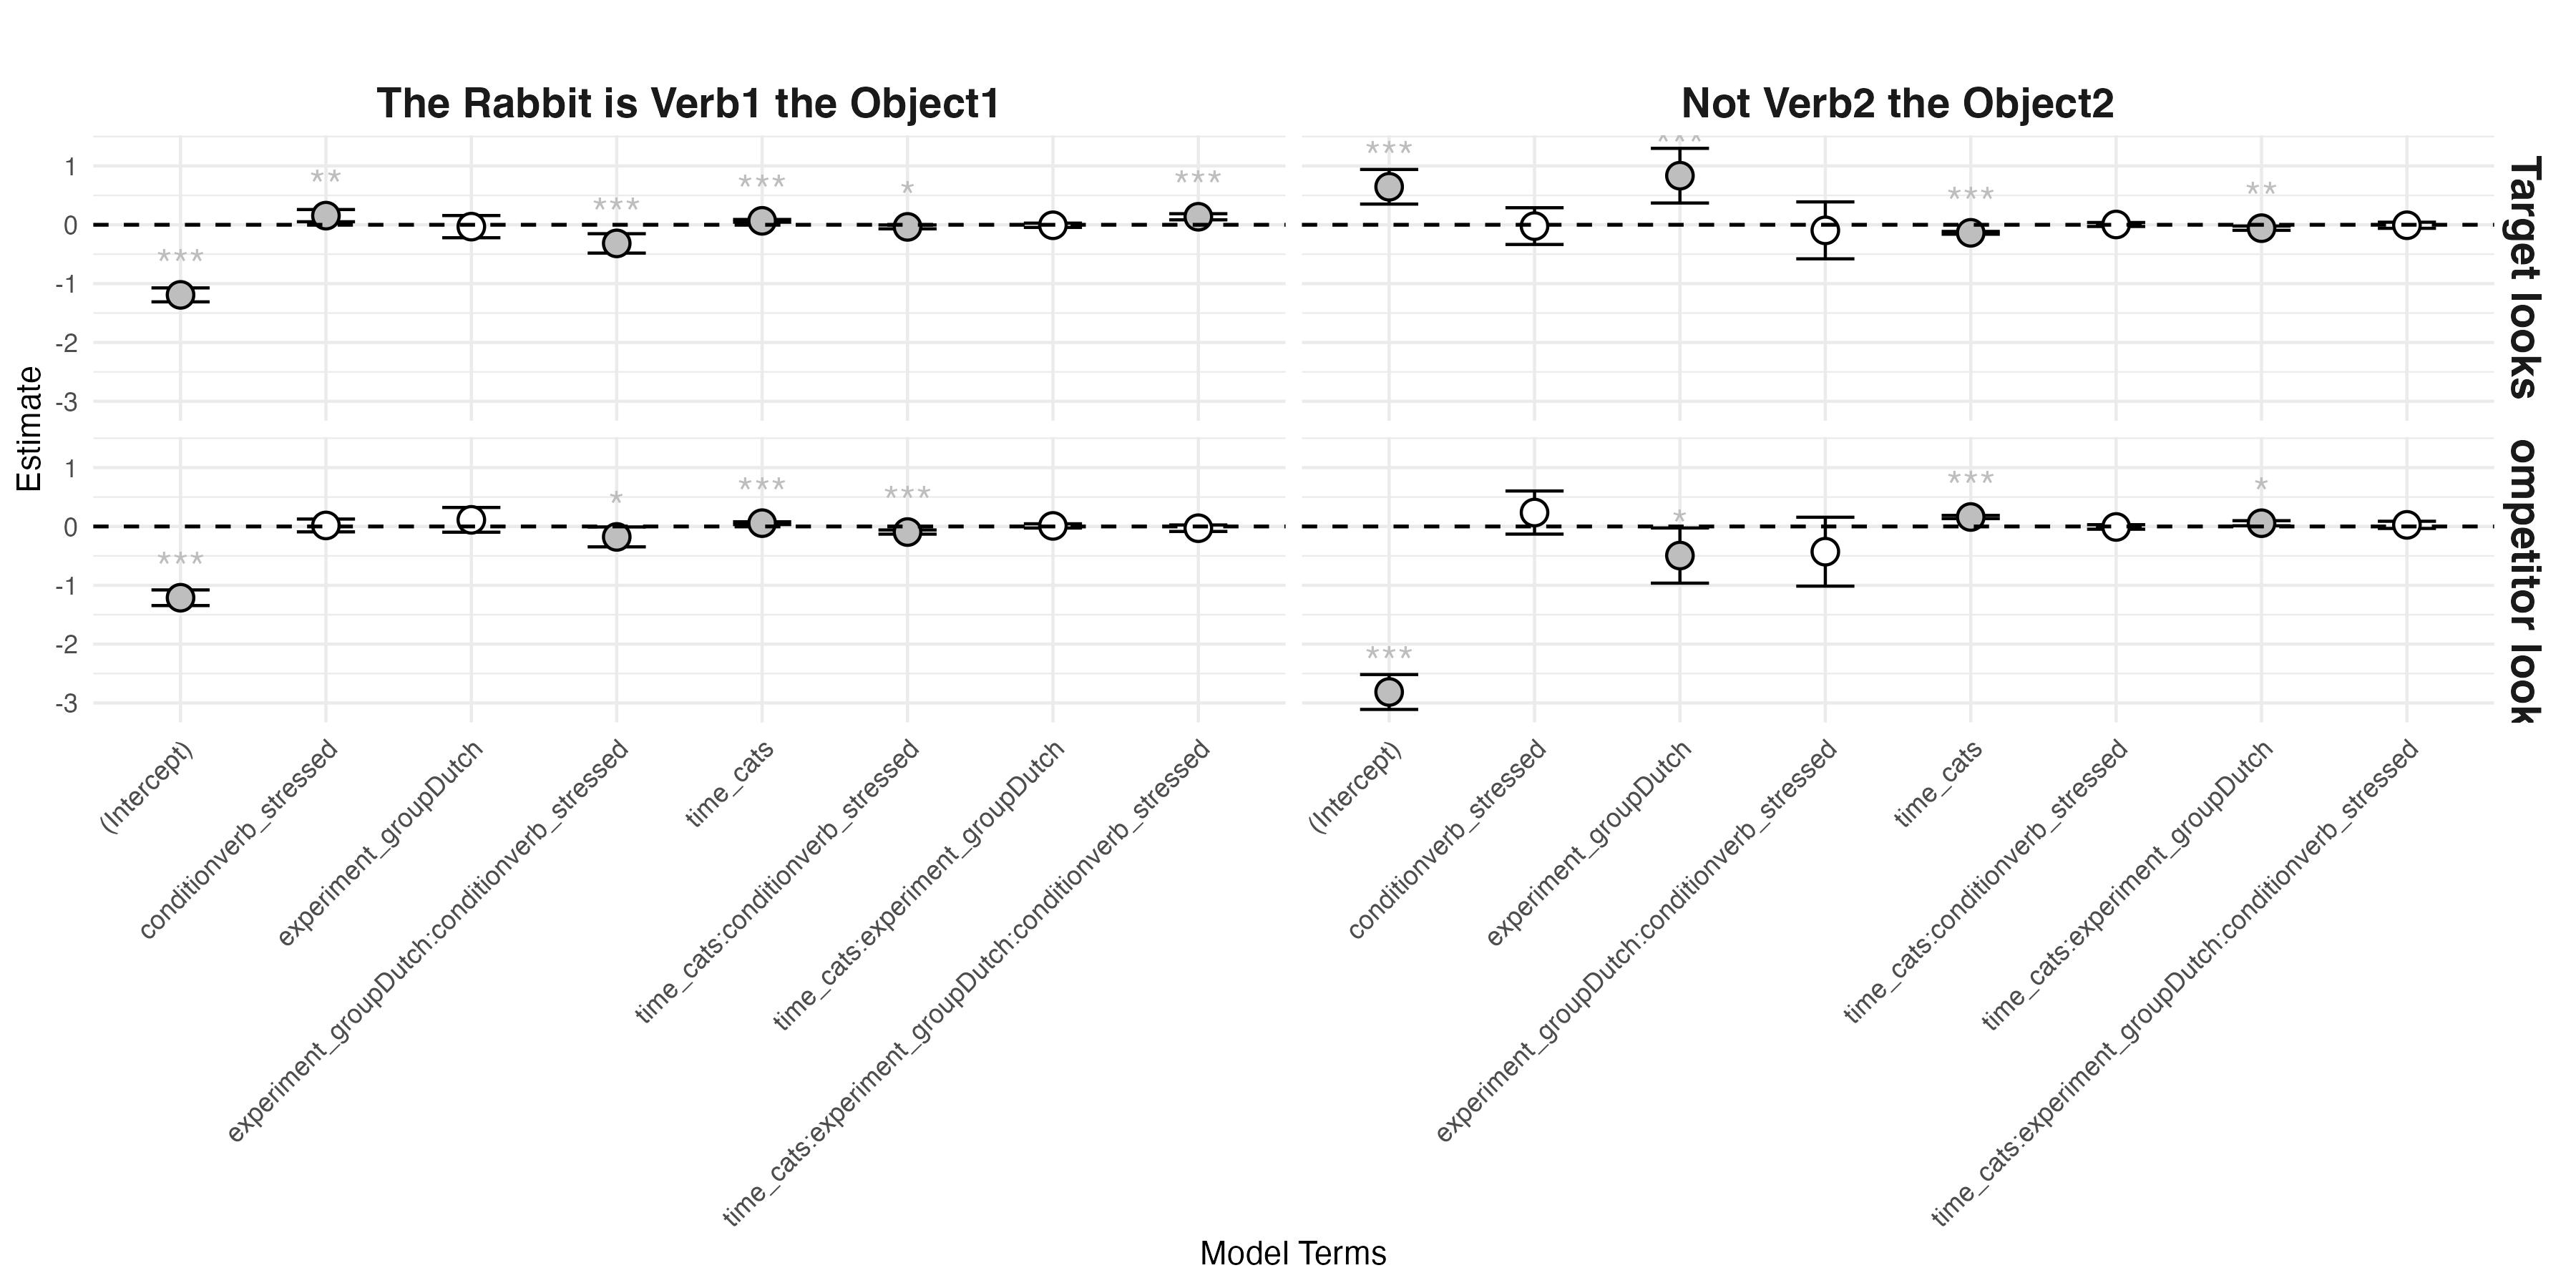
\includegraphics[width=\textwidth,height=\textheight,keepaspectratio]{viz/id_gam_mod_out.png}
    \caption{describe what is going on here- colorized by individual difference measure. Only significant variables are colored (white indicates non-significance). Grey indicates significant but not and individual difference measure}
    \label{fig:id_gam_mod_out}
\end{figure}

This exploratory extension allows us to assess the generalizability of the original findings by considering sources of variability that were not accounted for in the original study. Unlike the fidelity and refinement analyses, which adhere to confirmatory statistical approaches, this extension adopts a theory-driven, exploratory framework. We incorporate measures of lexical proficiency, auditory sensitivity, and motor reproduction ability to determine whether individual cognitive and perceptual traits predict variation in focus processing.

By adopting this three-tiered approach—fidelity, refinement, and extension—we provide a comprehensive analysis that both evaluates and expands upon the findings of \cite{Ge2021}. In what follows, we first present the results of our close replication, followed by methodological refinements, and finally, our exploratory analyses of individual differences.



